\documentclass[a4paper,12pt, openany]{book}
\usepackage[utf8]{inputenc}
\usepackage[T1]{fontenc}
\usepackage[portuguese]{babel}
\usepackage{amsmath, amssymb, amsthm}
\usepackage{graphicx}
\usepackage{hyperref}
\usepackage{color}
% \usepackage{anysize} 
%     \marginsize{2cm}{2cm}{2cm}{2cm}
\usepackage[a4paper, top=3cm, bottom=2.5cm, left=2cm, right=2cm]{geometry}
\usepackage{fancyhdr}
\usepackage{titlesec}
\usepackage{setspace}

\usepackage{cancel}
\usepackage{textcomp}
\usepackage{subcaption}
\usepackage{float}
\usepackage{tikz}
\usepackage{wrapfig}
\usepackage{multicol}


\usepackage[most]{tcolorbox} % For the example box
\tcbuselibrary{theorems}
\newcounter{example}[chapter]

\newtcolorbox[use counter=example]{examplebox}[1][]{
  colback=blue!5!white,       % Light blue background
  colframe=blue!40!black,     % Darker blue frame
  opacityframe=0.8,
  fonttitle=\bfseries,
  title={Exemplo \thechapter.\arabic{example}: #1},
  label={ex:#1},
  before skip=10pt,
  after skip=10pt,
  breakable,
  enhanced
}
  
\newcounter{history}[chapter]

\newtcolorbox[use counter=history]{historybox}[1][]{
  colback=red!5!white,       % Light blue background
  colframe=red!40!black,         % Moldura vermelha escura
  opacityframe=0.8,
  fonttitle=\bfseries,
  title={Nota histórica \thechapter.\arabic{history}: #1},
  label={hb:#1},
  before skip=10pt,
  after skip=10pt,
  breakable,
  enhanced
}

\newtheoremstyle{mystyle}% custom style name
{10pt}   % Space above
{10pt}   % Space below
{\itshape}  % Body font
{}       % Indent amount
{\bfseries} % Theorem head font
{.}      % Punctuation after theorem head
{.5em}   % Space after theorem head
{\thmname{#1}\thmnumber{ #2}\thmnote{ (#3)}}


\theoremstyle{mystyle}
\newtheorem{theorem}{Enunciado}[chapter]

\titleformat{\chapter}[display]
  {\normalfont\huge\bfseries}{\chaptertitlename\ \thechapter}{20pt}{\Huge}
\titlespacing*{\chapter}{0pt}{-20pt}{40pt}

% \setlength{\headheight}{16pt}
% \fancyhf{}
% \fancyhead[LE]{\textit{\leftmark}}
% \fancyhead[RO]{\textit{\rightmark}}
% \fancyfoot[C]{\thepage}
% \pagestyle{fancy}


\newcommand{\eqn}[2]{
    \textbf{#1}
    \begin{flalign*}
        #2
    \end{flalign*}
}


\title{Termodinâmica I}
\author{Gabriel Leitão}
\date{\today}

\begin{document}

\frontmatter
\begin{titlepage}
    \centering
    
\includegraphics[width=0.5\textwidth]{images/ist.jpg} % Opcional
    \vspace{2cm}

    {\Huge \bfseries Termodinâmica I\par}
    \vspace{1.5cm}
    {\Large \textit{Sebenta para Engenharia}\par}
    \vfill

    {\Large Gabriel Leitão\par}
    \vspace{0.5cm}
    {\large Instituto Superior Técnico\par}
    \vspace{0.5cm}
    {\large Junho 2025\par}
\end{titlepage}


\chapter*{Resumo}
Este texto enquadra-se na unidade curricular de Termodinâmica I de 2024/2025 de LEAer, LEAmb, LEMec, LEAN, no Instituto Superior Técnico. 

A termodinâmica é uma das disciplinas científicas mais fundamentais e abrangentes. O seu desenvolvimento ao longo dos séculos não apenas revolucionou a ciência, mas também transformou a tecnologia e a indústria, impulsionando a Revolução Industrial e moldando o mundo moderno.

Inspirada no livro \emph{Fundamentals of Engineering Thermodynamics} (Shapiro) \cite{shapiro}, esta sebenta integra também conteúdos lecionados em aula, organizados de forma a facilitar uma aprendizagem mais eficaz ao longo do período letivo. Inclui ainda exemplos resolvidos e notas históricas que contribuem para uma compreensão mais intuitiva dos conceitos.

Os ficheiros da sebenta estão disponíveis num repositório no GitHub: \url{https://github.com/GabrieLeitao/sebenta-termo} para quem quiser contribuir com correções ou melhorias, assegurando a atualização e continuidade da sebenta.


\vspace{1cm}
Revisão: Gabriel Faria
\vspace{1cm}

20 de Junho de 2025

\tableofcontents

\mainmatter


\chapter{Introdução à Mecânica dos Fluidos}
A mecânica dos fluidos é o ramo da física que estuda o comportamento de fluidos em repouso ou em movimento. Neste capítulo, é feita uma introdução dos conceitos fundamentais que serão úteis.

\section{Definição de fluido}

Um fluido é uma substância que se deforma continuamente quando sujeita a uma tensão de cisalhamento, por menor que ela seja. Ao contrário dos sólidos, que mantêm uma forma rígida, os fluidos não possuem forma própria e adaptam-se completamente ao recipiente que os contém.

Os fluidos podem ser classificados em \textbf{Líquidos} e \textbf{Gases}. Gases são compressíveis, enquanto os líquidos são geralmente considerados incompressíveis.

\section{Propriedades dos Fluidos}

\subsection{Pressão}

A pressão (\( p \)) é outra propriedade importante dos fluidos. Ela é definida como a força \( F \) exercida perpendicularmente por unidade de área \( A \):
\begin{equation*}
    p = \frac{F}{A}
\end{equation*}

A pressão é uma grandeza escalar, o que significa que ela não possui direção, mas sim um valor em cada ponto do fluido. Quando consideramos um fluido em equilíbrio, a pressão exerce-se igualmente em todas as direções (um princípio fundamental descrito por Pascal).

\section{Estática dos Fluidos}

Hidrostática é o ramo da Física que estuda o comportamento dos fluidos em repouso, analisando como propriedades como a pressão variam com a profundidade, e das forças exercidas pelos fluidos sobre superfícies imersas e recipientes.

\subsection{Lei de Stevin}

Considerando um fluido incompressível com densidade constante \( \rho \) e sujeito à aceleração gravítica \( g \), numa coluna vertical de altura \( z \) e área de secção transversal \( A \). A pressão \( p \) em qualquer ponto dentro desta coluna é a soma da pressão atmosférica \( p_0 \) e a pressão exercida pelo peso do fluido acima desse ponto.

O peso \( F \) da coluna de fluido é dado por:

\begin{equation*}
    F = m g = \rho g V = \rho g A z
\end{equation*}

A pressão \( p \) da coluna de fluido é dada por:

\begin{equation*}
    p = \frac{F}{A} = \frac{\rho g A z}{A} = \rho g z
\end{equation*}

Então, a pressão total é dado pela \textbf{Lei de Stevin}:

\begin{equation}
    p(z) = p_0 + \rho g z
\end{equation}

Como esperado, a pressão aumenta com a profundidade, já que o peso da coluna de fluido acima de um determinado ponto aumenta à medida que a profundidade aumenta. Além disso, sabemos que a pressão é também diretamente proporcional à densidade do fluido, à aceleração gravítica.

\begin{historybox}[O Barril de Pascal]

Blaise Pascal demonstrou, no século XVII, que a pressão em um fluido transmite-se igualmente em todas as direções. Na famosa experiência do barril, ele ligou um tubo vertical fino a um barril cheio de água. Ao adicionar água ao tubo, a pressão no fundo do barril aumentou a ponto de este explodir, mesmo com uma pequena quantidade de água extra. Esta experiência ilustra a lei de Stevin e a transmissão de pressões.

\end{historybox}


\section{Dinâmica dos Fluidos}

\subsection{Equação da Continuidade}

Ao acompanharmos um elemento material de fluido ao longo de um escoamento unidimensional, sabemos pelo princípio da conservação da massa, que em dois pontos do escoamento: $d m_1 = d m_2$, podendo, no entanto, o seu volume variar em regiões com diferentes densidades.

Em regime estacionário, onde as propriedades de um fluido não variam ao longo do tempo ($\frac{\partial \rho}{\partial t} = 0$ e $\frac{\partial \mathbf{v}}{\partial t} = 0$), sabendo que $dm = \rho \,dV$, temos que $\rho_1 dV_1 = \rho_2 dV_2$. Como num fluido unidimensional $dV = A dx$, obtemos $\rho_1 A_1 dx_1 = \rho_2 A_2 dx_2 \Longleftrightarrow \rho_1 A_1 \mathbf{v}_1 dt = \rho_2 A_2 \mathbf{v}_2 dt$, dado que $dx = \mathbf{v} \, dt$.

Desta forma, chegamos à equação da continuidade:

\begin{equation}
    \rho_1 A_1 \mathbf{v}_1= \rho_2 A_2 \mathbf{v}_2
\end{equation}

Para fluidos incompressíveis, $\rho = \text{const.}$:

\begin{equation}
    A_1 \mathbf{v}_1= A_2 \mathbf{v}_2
\end{equation}

Esta relação permite compreender que, por exemplo, num afunilamento do escoamento — como numa mangueira de jardim ou num bocal convergente —, se $A_2 < A_1$, então necessariamente $\mathbf{v}_2 > \mathbf{v}_1$.

Assim, a equação da continuidade exprime o princípio da \textbf{conservação da massa} no escoamento de um fluido. Na forma diferencial geral, válida para escoamentos compressíveis ou incompressíveis, é escrita como:

\begin{equation}
    \frac{\partial \rho}{\partial t} + \nabla \cdot (\rho \vec{\mathbf{v}}) = 0
\end{equation}

Esta equação indica que a variação temporal da densidade \(\rho\) num ponto é oposta à divergência do fluxo de massa nesse ponto:

\begin{equation} \notag
    \frac{\partial \rho}{\partial t} = - \nabla \cdot (\rho \vec{\mathbf{v}})
\end{equation} 

\begin{itemize}
    \item Se \(\nabla \cdot (\rho \vec{\mathbf{v}}) > 0\), sai mais fluido do que entra, e a densidade local diminui.
    \item Se \(\nabla \cdot (\rho \vec{\mathbf{v}}) < 0\), entra mais fluido do que sai, e a densidade local aumenta.
\end{itemize}

Para um fluido incompressível, a equação da continuidade reduz-se a:
\begin{equation*}
    \nabla \cdot \vec{\mathbf{v}} = 0
\end{equation*}
Fisicamente, isto significa que o volume de fluido que entra numa região é igual ao volume que sai dessa mesma região.


\subsection{Equação de Bernoulli}

A equação de Bernoulli descreve a conservação de energia ao longo de uma linha de corrente. Esta equação é derivada a partir da equação de Euler para escoamentos invíscidos (sem efeitos viscosos), estacionários e incompressíveis. Em escoamentos viscosos, há dissipação de energia devido ao atrito viscoso.

Considere duas secções transversais de um escoamento, nos pontos 1 e 2, com áreas \(A_1\) e \(A_2\), situadas a alturas \(z_1\) e \(z_2\) e sujeitas a pressões \(p_1\) e \(p_2\). Segue-se um elemento de volume \(dV\) que se desloca entre esses dois pontos num intervalo de tempo \(dt\), assumindo fluido incompressível. Sabemos que \(dV = A_1 dx_1 = A_2 dx_2\) e, pela equação da continuidade, \(A_1 \mathbf{v}_1 = A_2 \mathbf{v}_2\).

O trabalho das forças de pressão sobre o elemento de volume é dado por:
\begin{align*}
    W_p & = F_1 dx_1 - F_2 dx_2 \\
    & = p_1 A_1 dx_1 - p_2 A_2 dx_2 = (p_1 - p_2) dV
\end{align*}

O trabalho realizado pela força da gravidade sobre o elemento é igual ao simétrico da variação da energia potencial gravitacional:

\begin{align*}
    W_g &= - m g \Delta z \\
    &= - \rho g (z_2 - z_1) dV
\end{align*}

A variação da energia cinética do elemento de volume é:
\begin{equation*}
    \Delta E_c = \frac{1}{2} \rho dV (\mathbf{v}_2^2 - \mathbf{v}_1^2)
\end{equation*}

Assim, pela conservação da energia mecânica para o elemento de fluido, temos: $W_p + W_g = \Delta E_c$

\begin{equation*}
    (p_1 - p_2) dV - \rho g (z_2 - z_1) dV = \frac{1}{2} \rho dV (\mathbf{v}_2^2 - \mathbf{v}_1^2)
\end{equation*}

Ou seja, rearranjando os termos:

\begin{equation}
    p_1 + \frac{1}{2} \rho \mathbf{v}_1^2 + \rho g z_1 = p_2 + \frac{1}{2} \rho \mathbf{v}_2^2 + \rho g z_2  
\end{equation}    

ou, genericamente, ao longo da linha de corrente:

\begin{equation}
    p + \frac{1}{2} \rho \mathbf{v}^2 + \rho g z = \text{const.}
\end{equation}

Isto implica que, se a velocidade do fluido aumenta, a pressão ou a altura do fluido deve diminuir para que a energia total se mantenha constante.

No caso da asa de um avião, a velocidade do ar sobre o extradorso é maior do que no intradorso, o que resulta numa pressão mais baixa na superfície superior comparativamente à inferior. Este diferencial de pressão gera a força de sustentação que permite o voo.


\begin{examplebox}[Limite de succção de bombas centrífugas de água]

As bombas centrífugas de água aceleram o fluido da zona central para a periferia do rotor, onde a área do escoamento diminui, implicando, pela equação da continuidade, um aumento da velocidade (\(A \downarrow \implies \mathbf{v} \uparrow\)). 

Pela equação de Bernoulli, um aumento da velocidade está associado a uma diminuição da pressão (\(\mathbf{v} \uparrow \implies p \downarrow\)), pelo que a bomba cria uma baixa pressão na zona central. 

Esta diferença entre a pressão atmosférica a que a água está sujeita no reservatório (por exemplo, um poço) e a baixa pressão no interior da bomba permite que a água suba pelo tubo até à bomba.

No entanto, existe uma limitação física para a altura máxima da coluna de água que a bomba consegue aspirar, dada por:

\begin{equation*}
    h = \frac{p_0}{\rho g} = \frac{101325}{1000 \times 9,81} \approx 10{,}3 \; \mathrm{m}
\end{equation*}

Para atingir essa altura seria necessário criar um vácuo perfeito, algo impossível numa bomba real. Na prática, o limite situa-se em cerca de 7 m, pois a pressão interna não deve ser inferior à pressão de saturação da água, para evitar a vaporização do fluido, fenómeno que pode causar cavitação e danificar a bomba.

Adicionalmente, a bomba converte energia cinética do movimento de rotação em pressão estática, fazendo sair o fluido com elevada pressão e velocidade.

\end{examplebox}

\begin{historybox}[O Tubo de Pitot]

Henri Pitot desenvolveu um dispositivo para medir a velocidade de escoamento com base na equação de Bernoulli. O tubo de Pitot é amplamente utilizado em aeronaves e sistemas de medição de fluidos. O dispositivo mede a diferença de pressão entre a extremidade aberta do tubo ($p_{total}$) e a extremidade da medição ($p_{estatica}$), a partir da qual se pode determinar a velocidade do fluido: $p_{total} = p_{estatica} + \frac{1}{2} \rho \mathbf{v}^2$, pelo que a velocidade é $\mathbf{v} = \sqrt{\frac{2 \Delta p}{\rho}}$.

\end{historybox}


\begin{historybox}[Torricelli e o vácuo]

Evangelista Torricelli (1608--1647), físico e matemático italiano, realizou uma experiência fundamental para a termodinâmica, desafiando a visão aristotélica do \textit{horror vacui} — a crença de que o vácuo não podia existir.

Em 1643, Torricelli usou um tubo de vidro com cerca de 1 metro, fechado numa extremidade, que encheu com mercúrio (devido à sua elevada densidade). Tapou a extremidade aberta com o dedo, inverteu o tubo e mergulhou-o numa tina com mercúrio. Ao retirar o dedo, o mercúrio desceu mas estabilizou a cerca de 760 mm acima do nível da tina, criando no topo do tubo o \textbf{vácuo torricelliano}.

Torricelli concluiu que o mercúrio era sustentado pela pressão atmosférica sobre o líquido na tina, afirmando:

\begin{quote}
    ``Vivemos submersos no fundo de um oceano do elemento ar, que por experiências inquestionáveis se sabe ter peso.''
\end{quote}


Esta descoberta criou o primeiro barômetro, permitindo a medição da pressão atmosférica.
\begin{equation*}
    p_{atm} = \rho_{Hg} \, g \, h
\end{equation*}

A altura da coluna de mercúrio na experiência de Torricelli pode ser calculada, sabendo a densidade do mercúrio $\rho_{Hg} = 13595.1~\text{kg/m}^3$ (a 0\textdegree C).

\begin{equation*}
    h = \frac{101325~\text{Pa}}{13595.1~\text{kg/m}^3 \cdot 9.80665~\text{m/s}^2} \approx 0.76~\text{m} = 760~\text{mm}
\end{equation*}
Esta altura de 760 mm de mercúrio tornou-se a definição da unidade de pressão \textbf{milímetros de mercúrio} (mmHg) ($1~\text{atm} = 101325~\text{Pa} = 760~\text{mmHg}$).

\textbf{Blaise Pascal} estendeu o trabalho de Torricelli, demonstrando que a pressão atmosférica diminui com a altitude. Para isso pediu ao cunhado \textbf{Florin Périer} para medir a pressão atmosférica a diferentes altitudes no Puy de Dôme em 1648, com uma coluna de mercúrio. Uma coluna de água seria impraticável, pois exigiria cerca de $10.3~\text{m}$ de altura.

\end{historybox}

\begin{historybox}[Otto von Guericke e a força do vácuo]

Inspirado por Torricelli, \textbf{Otto von Guericke}, um cientista alemão dedicou-se a investigar o vácuo. Em 1649, Otto von Guericke desenvolveu a primeira bomba de vácuo, um dispositivo capaz de extrair ar de um recipiente selado, criando um vácuo parcial. 

Para demonstrar o poder do vácuo e a força da pressão atmosférica, Guericke realizou, em 1654, a célebre experiência dos Hemisférios de Magdeburgo. Nela, duas semiesferas de cobre com 20 polegadas, cerca de 50 cm, de diâmetro foram unidas e o ar do interior foi removido com a bomba. A pressão atmosférica externa tornou impossível separá-las. Numa demonstração pública em Regensburg, diante do Imperador Fernando III, duas equipas com oito cavalos cada tentaram — sem sucesso — separar os hemisférios.

\end{historybox}

\subsection{Equação de Navier-Stokes}

A equação de Navier-Stokes descreve o movimento de fluidos viscosos e é a equação fundamental para os fluidos não ideais. Ela é dada por:
\begin{equation}
    \rho \left( \frac{\partial \vec{\mathbf{v}}}{\partial t} + (\vec{\mathbf{v}} \cdot \nabla) \vec{\mathbf{v}} \right) = -\nabla p + \mu \nabla^2 \vec{\mathbf{v}} + \vec{f}
\end{equation}

onde \( \vec{f} \) representa as forças externas (como a gravidade).

Esta equação é derivada das leis de Newton e expressa o equilíbrio entre a inércia, as forças de pressão, as forças viscosas e as forças externas. Resolver as equações de Navier-Stokes é um dos maiores desafios na física e na matemática, sendo parte dos Problemas do Prêmio Millennium do Clay Institute.

Desprezando o termo viscoso (\(\mu = 0\)), obtém-se a equação de Euler:

\begin{equation}
    \rho \left( \frac{\partial \vec{\mathbf{v}}}{\partial t} + (\vec{\mathbf{v}} \cdot \nabla) \vec{\mathbf{v}} \right) = -\nabla p + \vec{f}
\end{equation}

Supondo escoamento incompressível e estacionário (\(\partial/\partial t = 0\)) e tomando \(\vec{f} = \rho \vec{g}\), pode-se obter, novamente, a equação de Bernoulli:

\begin{equation*}
    \rho (\vec{\mathbf{v}} \cdot \nabla) \vec{\mathbf{v}} = -\nabla p + \rho \vec{g}
\end{equation*}

Projectando ao longo de um deslocamento infinitesimal \(d\vec{s}\), para a linha de corrente:

\begin{eqnarray*}
    \rho \vec{\mathbf{v}} \cdot d\vec{\mathbf{v}} = -dp + \rho \vec{g} \cdot d\vec{s} \\
    \rho d \left(\frac{\mathbf{v}^2}{2}\right) = -dp - \rho g dz \\
    d \left( p + \frac{1}{2} \rho \mathbf{v}^2 + \rho g z \right) = 0
\end{eqnarray*}

\chapter{Introdução}
\section{Conceitos e Definições}

O \textbf{sistema} identifica o objeto de estudo de uma análise termodinâmica. Um sistema pode ser \textbf{aberto}, \textbf{fechado} ou \textbf{isolado}. Um sistema fechado refere-se a uma quantidade de matéria fixa, enquanto um sistema aberto, ou volume de controlo, é uma região do espaço pelo qual pode haver transferências de massa pela fronteira. Em ambos, pode haver transferência de energia. Num sistema isolado, não há interação com a vizinhança. Sistemas isolados não ocorrem naturalmente.

A fronteira de um sistema pode ser: \textbf{adiabática}, quando não permite trocas de calor (\textbf{diatérmico}, caso contrário); \textbf{rígida}, quando não permite execução de trabalho, ou \textbf{móvel}, caso contrário. Aquilo que está para além da fronteira, é considerada a \textbf{vizinhança}.

Uma \textbf{propriedade} é uma grandeza macroscópica do sistema num dado instante, cujo valor pode ser determinado independentemente da história anterior do sistema.

Um \textbf{estado} é a condição do sistema descrita pelas suas propriedades. O estado de um sistema pode ser determinado por um subconjunto mínimo das suas propriedades, a partir do qual as restantes podem ser determinadas. Por exemplo, para gases ideais, basta 2 propriedades independentes para definir o estado do sistema.

Diz-se que ocorreu um \textbf{processo}, quando uma ou mais propriedades variam, e consequentemente muda o estado do sistema. 

\begin{quote}
    ``Uma quantidade é uma propriedade se e só se a sua variação entre dois estados é independente do processo.''
\end{quote}


Num \textbf{estado estacionário} as propriedades não variam com o tempo. Um \textbf{estado de equilíbrio} implica que não ocorram processos espontâneos que façam o sistema mudar de estado. Um sistema que, ao ser isolado, não sofre quaisquer alterações, implica que estava em equilíbrio quando foi isolado.

Um processo pode ser: \textbf{isotérmico}, se ocorre a temperatura constante; \textbf{isobárico}, se ocorre a pressão constante; e \textbf{isocórico}, se ocorre a volume constante.

As propriedades podem ser \textbf{extensivas} se dependem do tamanho do sistema, como a massa, o volume, a energia, e a entropia. O valor de uma propriedade extensiva de um sistema é igual à soma do valor da propriedade de todas as partes que compõem o sistema, ou seja, são funções do tempo. Por outro lado, as propriedades que são função do tempo e do espaço, como a pressão, a temperatura e o volume específico, denominam-se propriedades \textbf{intensivas}. Por exemplo, a massa de um conjunto de peças é igual à soma das massas de cada peça individualmente, mas a temperatura do conjunto não é a soma das temperaturas de cada peça.

Entre dois sistemas podem existir transferências de energia, que resultam de \textbf{calor} ou \textbf{trabalho}. O calor e o trabalho não são funções contínuas, mas apenas podem ser quantificados como a energia total transferida dessa forma entre dois estados, devido a um dado processo.

Um \textbf{reservatório térmico}, ou apenas reservatório, é um sistema que se mantém a temperatura constante, mesmo que receba ou ceda energia por calor. Deste modo, um reservatório é uma idealização de corpos grandes, como a atmosfera, grandes corpos de água (lagos, oceanos), ou sistema de duas fases a pressão constante. Propriedades extensivas como a energia interna podem variar.

Um \textbf{ciclo} é uma sequência de processos que começa e acaba no mesmo estado. Desta forma, no final de um ciclo ideal, todas as propriedades do sistema retornarão ao valor inicial.

\subsection{Propriedades}

Quando as substâncias são um contínuo, pode-se falar de propriedades intensivas num ponto. Por exemplo, a \textbf{densidade} $\rho$ em cada ponto pode ser definida:

\begin{equation}
    \rho = \lim_{V \to V'} \frac{m}{V}
\end{equation}

onde $V'$ é o menor volume para o qual existem partículas suficientes para médias estatísticas, e para o qual a matéria pode ser considerado um contínuo. 

A densidade é, portanto, uma propriedade intensiva que pode variar de ponto para ponto. O \textbf{volume específico} é o inverso da densidade, $v = \frac{1}{\rho}$, que igualmente, depende da posição e é uma propriedade intensiva. As unidades SI são $\text{m}^3 / \text{kg}$.

A massa pode ser determinada por integração, sabendo $\rho$. Quando a densidade é uniforme, então $m = \rho V$.

\begin{equation}
    m = \int_{V} \rho \, dV
\end{equation}

Considerando uma área pequena \( A \) num ponto de um fluido em repouso, o fluido exerce sobre essa área uma força compressiva \( F \), normal a \( A \). Pelo princípio da ação e reação, do outro lado da área o fluido exerce uma força igual e oposta, mantendo o equilíbrio estático.
A \textbf{pressão} nesse ponto é definida como:

\begin{equation}
    p = \lim_{A \to A'} \frac{F}{A}
\end{equation}

onde $A'$ tem o mesmo significado de ponto limite usado na definição de densidade, e $F$ a força normal a essa área.

\subsubsection{Conversão de unidades de pressão}

\begin{eqnarray*}
    1 \; \text{Pa} = 1 \; \text{N}/\text{m}^2       \\
    1 \; \text{kPa} = 10^3 \; \text{N}/\text{m}^2   \\
    1 \; \text{bar} = 10^5 \; \text{N}/\text{m}^2   \\
    1 \; \text{atm} = 101325 \; \text{N}/\text{m}^2 \\
    1 \; \text{MPa} = 10^6 \; \text{N}/\text{m}^2   
\end{eqnarray*}

\chapter{Primeira Lei da Termodinâmica}

\begin{theorem}[Lei Zero da Termodinâmica]
    Quando dois objetos estão em equilíbrio térmico com um terceiro objeto, os dois estão em equilíbrio térmico entre si.
\end{theorem}

\section{Balanço de Energia}

A partir das contribuições de Galileu e outros, Newton formulou as leis do movimento, fundamentais na mecânica.

Considerando a força tangencial ao movimento e $\mathbf{v} = \frac{ds}{dt}$:

\begin{eqnarray*}
    F = m \frac{d\mathbf{v}}{dt} = m \frac{d\mathbf{v}}{ds} \frac{ds}{dt} = m \mathbf{v} \frac{d\mathbf{v}}{ds} \\
    \int_{\mathbf{v}_1}^{\mathbf{v}_2} m \mathbf{v} \, d\mathbf{v} = \int_{s_1}^{s_2} F \, ds \\
    \Delta E_c = \frac{1}{2} m \left( \mathbf{v}_2^2 - \mathbf{v}_1^2 \right) = \int_{s_1}^{s_2} F \, ds
\end{eqnarray*}

Ou seja, o trabalho de uma força ao longo da trajetória equivale à variação da energia cinética.

Seja $R$ a força resultante exceto a gravítica, com $g$ constante:

\begin{eqnarray*}
    \frac{1}{2} m \left( \mathbf{v}_2^2 - \mathbf{v}_1^2 \right) = \int_{s_1}^{s_2} R \, ds - \int_{z_1}^{z_2} mg \, dz \\
    \Delta E_p = mg(z_2 - z_1) \\
    \int_{s_1}^{s_2} R \, ds = \Delta E_c + \Delta E_p
\end{eqnarray*}

As energias cinética e potencial são propriedades extensivas do sistema, com unidades de energia, iguais às do trabalho: em SI, sendo $W = \int \vec{F} \cdot d\vec{s}$, o trabalho tem unidades $\text{N} \cdot \text{m}$, que se denomina Joule, J.

O \textbf{trabalho} é uma forma de transferir energia. O trabalho $W$ depende nos detalhes das interações a ocorrer entre um sistema e a vizinhança num determinado processo, pelo que o trabalho não é uma propriedade. O diferencial de trabalho, $\delta W$, é inexato: $\int_1^2 \delta W = W$. Por outro lado, o diferencial de uma propriedade é exato. Por exemplo, para o volume: $\int_{V_1}^{V_2} dV = V_2 - V_1$.

A taxa com que dada transferência de energia ocorre, fruto de trabalho, denomina-se \textbf{potência}, $\dot{W}$, unidade SI é o Watt, W.

\begin{eqnarray*}
    \dot{W} = \frac{d}{dt} \int \vec{F} \cdot d\vec{s} = \vec{F} \cdot \vec{\mathbf{v}}\\
    W = \int \dot{W} dt
\end{eqnarray*}

\subsection{Trabalho de Compressão/Expansão}

Neste texto, convenciona-se que qualquer forma de energia que entra no sistema é positiva e energia que sai é negativa, \textbf{seguindo a convenção nas aulas, contrária à do Shapiro}.

Considerando um sistema êmbolo-cilindro, a pressão do gás exerce uma força no pistão, durante a expansão. O trabalho feito pelo sistema quando o êmbolo se move é:  

\begin{equation*}
    \delta W = - F \, dx = - pA \, dx \implies \delta W = - p \,dV
\end{equation*}

Assim, o trabalho é dado por 

\begin{equation}
    W = - \int_{V_1}^{V_2} p \, dV
\end{equation}

Desta forma, tal como convencionado: durante uma expansão $dV > 0$ e $W < 0$, o sistema perde energia; enquanto numa compressão $dV < 0$ e $W > 0$, o sistema recebe energia.

A equação do trabalho é válida para sistemas de qualquer forma, desde que a pressão seja uniforme ao longo da fronteira móvel.

O módulo do trabalho corresponde à área sob a curva num diagrama $p$-$V$. Como diferentes processos entre os mesmos estados 1 e 2 podem gerar curvas distintas, o trabalho depende do processo realizado.

\subsubsection{Processo Politrópico}

Um processo de quase equilíbrio descrito por $pV^n = \text{const.}$ ou $pv^n = \text{const.}$, onde $n$ é uma constante, chama-se \textbf{processo politrópico}. 

O trabalho para um processo politrópico, onde $c = p V^n = p_1 V_1^n = p_2 V_2^n$ e $p = \frac{c}{V^n}$, é:

\begin{itemize}
    \item Para $n \neq 1$:
    \begin{equation*}
        \begin{split}
            W & = - \int_{V_1}^{V_2} \frac{c}{V^n} \, dV  = - \frac{c V_2^{1-n} - c V_1^{1-n}}{1-n} = \frac{(p_2 V_2^n) V_2^{1-n} - (p_1 V_1^n) V_1^{1-n}}{n - 1} \\
            W & = \frac{p_2 V_2 - p_1 V_1}{n - 1}, \quad n \neq 1
        \end{split}
    \end{equation*}
    \item Para $n = 1$:
    \begin{equation*}
        \begin{split}
            W & = - \int_{V_1}^{V_2} \frac{c}{V} \, dV  = - c \ln \frac{V_2}{V_1} \\
            W & = - p_1 V_1 \ln \frac{V_2}{V_1} = - p_2 V_2 \ln \frac{V_2}{V_1}, \quad n = 1
        \end{split}
    \end{equation*} 
\end{itemize}

Dado que $p_1V_1^n = p_2V_2^n$:

\begin{eqnarray}
    \frac{p_1}{p_2} = \left( \frac{V_2}{V_1} \right)^n \Longleftrightarrow 
    \ln \left( \frac{V_2}{V_1} \right)^n = \ln \frac{p_1}{p_2} \Longleftrightarrow 
    n \ln \frac{V_2}{V_1} = \ln \frac{p_1}{p_2} \implies
    n = \frac{\ln \frac{p_1}{p_2}}{\ln \frac{V_2}{V_1}}
\end{eqnarray}

\subsection{Energia Interna}

A variação da energia total de um sistema é calculada com base em três grandes contribuições: energia cinética, energia potencial -- associadas ao movimento e posição do sistema --, e \textbf{energia interna}, $U$, onde estão concentradas as outras contribuições. Todas estas energias são propriedades extensivas.
\begin{equation}
    \Delta E = \Delta U + \Delta E_c + \Delta E_p 
\end{equation}

Microscopicamente, a energia interna inclui: energia cinética translacional, rotacional e vibracional das moléculas; energia das ligações químicas; energia atómica (orbitais, spin) e nuclear. Em substâncias condensadas, as forças intermoleculares também contribuem significativamente para $U$.

\subsection{Calor}

Da mesma forma que o trabalho, o \textbf{calor} não é uma propriedade, pois depende do processo. $Q = \int_1^2 \delta Q$.
A taxa de transferência de energia por calor pode ser dada por:

\begin{equation*}
    \dot{Q} = \int_A \dot{q} \, dA
\end{equation*}

onde $\dot{q}$ é o fluxo de calor por unidade de área.

A transferência de calor pode ser por \textbf{condução} ou \textbf{radiação}, e uma combinação que produz a \textbf{convecção}.

\subsubsection{Condução}

A condução é a transferência de energia de moléculas mais energéticas de uma substância para partículas adjacentes.

A Lei de Fourier permite calcular a taxa de transferência de energia por condução:

\begin{equation}
    \dot{Q}_x = - \kappa A \frac{dT}{dx}, \quad \dot{\vec{Q}} = - \kappa A \nabla T
\end{equation}

onde $\kappa$ é uma constante chamada condutividade térmica. O sinal negativo reflete o facto da transferência ocorrer na direção de menor temperatura.

\subsubsection{Radiação}

A radiação transmite energia por ondas eletromagnéticas, fotões. Ao contrário da condução, a radiação pode transferir energia no vácuo.

A taxa de transferência de energia por radiação pode ser calculada por uma forma modificada da Lei de Stefan-Boltzmann:

\begin{equation}
    \dot{Q}_e = \epsilon \sigma A T^4
\end{equation}

onde $T$ é a temperatura da superfície, $\epsilon$ é a emissividade da superfície ($0 \leq \epsilon \leq 1$), e $\sigma = 5.67 \cdot 10^{-8} \; \text{W}/\text{m}^2 \cdot \text{K}^4$.

A emissividade $\epsilon$ é uma grandeza adimensional que quantifica a capacidade de uma superfície emitir radiação térmica em comparação com um corpo negro ideal ($\epsilon = 1$). Superfícies metálicas polidas, por serem altamente refletoras, têm baixa emissividade, enquanto superfícies negras ou rugosas apresentam valores próximos de $1$.

A emissividade depende do material, do estado da superfície, da temperatura e do comprimento de onda. Em muitos casos, utiliza-se uma emissividade média ou espetral para simplificação.


\subsubsection{Convecção}

A lei de arrefecimento de Newton dá-nos uma expressão experimental para calcular a transferência de energia por convecção de uma superfície sólida à temperatura de $T_b$ e um gás ou líquido adjacente a $T_f$.
\begin{equation}
    \dot{Q}_c = h A (T_b - T_f), \quad \dot{Q} = h A \Delta T
\end{equation}

onde $h$ é um coeficiente de transferência de calor, determinado experimentalmente, que depende do fluido, da geometria, da rugosidade da superfície e das condições de escoamento (como velocidade e regime laminar ou turbulento).


\subsection{Primeira Lei da Termodinâmica}

Joule demonstrou experimentalmente que a energia é conservada, i.e. a energia não pode ser criada ou destruída, apenas convertida. Isto é considerado a Primeira Lei da Termodinâmica.

Para um sistema fechado, Joule deduziu que o trabalho em qualquer processo adiabático entre dois estados de equilíbrio é o mesmo. Como depende apenas dos estados inicial e final, por definição de propriedade, esse trabalho corresponde à variação de uma propriedade do sistema, a energia, i.e., \(\Delta E = W_{\text{adia}}\).

Do \textbf{balanço de energia} geral resulta:

\begin{equation}
    \Delta E = \Delta E_c + \Delta E_p + \Delta U = Q + W
\end{equation}

Na forma diferencial:

\begin{equation}
    dE = \delta Q + \delta W, \qquad \frac{dE}{dt} = \frac{dE_c}{dt} + \frac{dE_p}{dt} + \frac{dU}{dt} = \dot{Q} + \dot{W}
\end{equation}

Recorrentemente, as energias cinéticas e potenciais macroscópicas do sistema são desprezáveis:

\begin{equation}
    \Delta U = Q + W, \qquad \frac{dU}{dt} = \dot{Q} + \dot{W}
\end{equation}


\section{Volumes de Controlo}

Para sistemas com fluxo de massa, existe transferência de energia associado ao trabalho do fluxo volumétrico que entra ou sai:

\begin{equation*}
    \frac{dE}{dt} = \vec{F} \cdot \vec{\mathbf{v}} = p A \mathbf{v} = p A \frac{dx}{dt} = p \frac{dV}{dt} = p \frac{v dm}{dt} = \dot{m} pv 
\end{equation*}

e o balanço energético para o volume de controlo é:

\begin{equation}
    \frac{dE}{dt} = \frac{dU}{dt} + \frac{dE_c}{dt} + \frac{dE_p}{dt} = \dot{Q} + \dot{W} + \sum_i \dot{m} \left( \frac{1}{2}\mathbf{v}_i^2 + gz_i + u_i + p_i v_i \right)
\end{equation}

Deste modo, define-se a \textbf{entalpia} como $h = u + pv$, uma grandeza útil para o estudo. Desprezando termos cinéticos e potenciais:

\begin{equation}
    \frac{dU}{dt} = \dot{Q} + \dot{W} + \sum_i \dot{m} h_i
\end{equation}

Muitas vezes a entalpia é muito maior comparativamente aos termos de energia cinética e potencial associada ao fluxo de massa que passa a fronteira do sistema ($h_i \gg \frac{1}{2}\mathbf{v}_i^2 + gz_i$), sendo, por isso, desprezáveis.

\chapter{Propriedades}

\section{Tabelas}

A água pode se encontrar em mudança de fase, por exemplo, na vaporização estão presentes duas fases, a fase líquida e a fase gasosa:

\begin{eqnarray}
    V = V_{liq} + V_{vap}\\
    v = \frac{V_{liq} + V_{vap}}{m}
\end{eqnarray}

onde $V_{liq} = m_{liq} v_f$ e $V_{vap} = m_{vap} v_g$, pelo que:

\begin{equation}
    v = \frac{m_{liq}}{m} v_f + \frac{m_{vap}}{m} v_g
\end{equation}

Definindo $x = \frac{m_{vap}}{m}$, como o título da água, temos $\frac{m_{liq}}{m} = 1 - x$ e podemos escrever:

\begin{equation}
    v = (1-x) v_f + x v_g = v_f + x(v_g - v_f)
\end{equation}

E, portanto,

\begin{equation}
    x = \frac{v-v_f}{v_g-v_f}
\end{equation}

\begin{figure}[H]
    \centering
    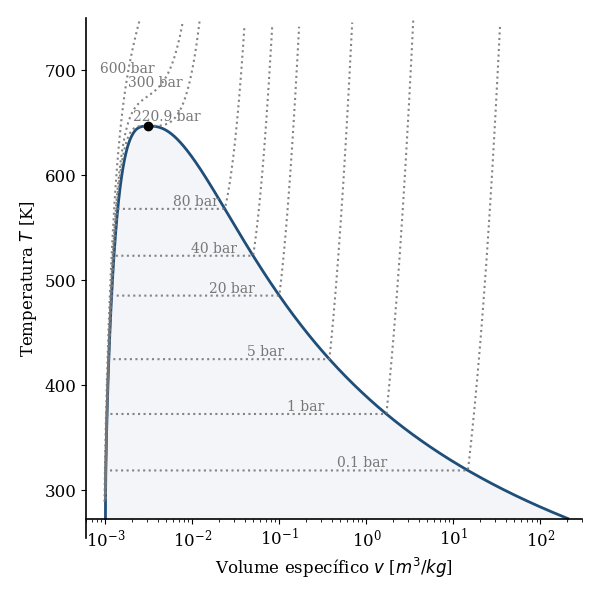
\includegraphics[width=0.4\linewidth]{graphs/water-dome-Tv-critical.png}
    \caption{Diagrama T-v da água}
    \label{fig:water-dome-Tv}
\end{figure}

É possível verificar que para uma pressão de $1.01325~\text{bar} = 1~\text{atm}$, a temperatura de saturação é $100~\text{\textdegree C} = 373.15~\text{K}$ -- i.e. a temperatura à qual ocorre a vaporização da água em condições de pressão atmosférica.

O ponto crítico da água ocorre a uma pressão de $p = 22.09~\text{MPa} = 220.9~\text{bar}$ e temperatura de $T = 647.096~\text{K}$.

Nas curvas de pressão constante -- \textbf{isobáricas} --, observa-se que, para pressões acima da pressão crítica, a temperatura aumenta continuadamente com o aumento do volume específico (os termos líquido e vapor perdem significado para estas pressões). 

Por outro lado, para pressões abaixo da pressão crítica, existe uma região bifásica, onde mantendo uma pressão fixa, a temperatura permanece constante durante a vaporização, enquanto o volume específico aumenta.

\begin{figure}[H]
    \centering
    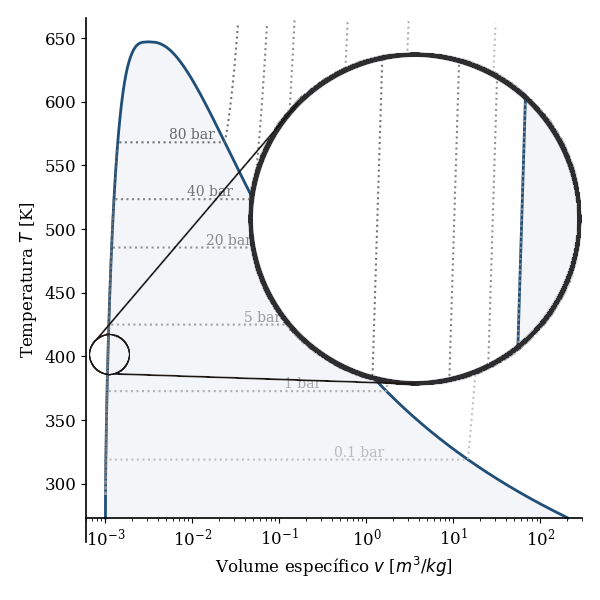
\includegraphics[width=0.4\linewidth]{graphs/water-dome-Tv-circle.png}
    \caption{Isobáricas no domo da água ampliadas}
    \label{fig:water-dome-Tv-amp}
\end{figure}

Neste gráfico consegue-se ver que para a água em líquido comprimido aproximar $u(T, p) \approx u_f(T)$, $h(T, p) \approx h_f(T)$, etc, é uma boa aproximação, já que $v \approx \text{const}$.

\begin{equation}
    u = (1-x) u_f + x u_g = u_f + x(u_g - u_f)
\end{equation}

\begin{equation}
    h = (1-x) h_f + x h_g = h_f + x(h_g - h_f)
\end{equation}

O aumento de entalpia durante a vaporização é $h_{fg} = h_g - h_f$, então: $h = h_f + x h_{fg}$.

\section{Escalas Termodinâmicas de Temperatura}

Existem duas escalas termodinâmicas de temperatura, ou seja, onde a temperatura menor é 0. Estas são a Escala de Kelvin e a Rankine.

\begin{equation}
    T(\text{\textdegree R}) = 1.8 \, T(\text{K})
\end{equation}

Por convenção internacional, as escalas de temperatura são definidas para o facilmente reproduzível ponto triplo da água - estado de equilíbrio entre vapor, gelo e água líquida. Este encontra-se a 273.16 K. O ponto de gelo da água (equilíbrio entre gelo e água saturada com ar) a 1 atm é 273.16 K até o ponto de equilíbrio de vapor e água líquida a 1 atm são 100 K.

A diferença de temperatura é igual na escala de Kelvin e na de Celsius. 

\begin{equation}
    T(\text{\textdegree C}) = T(\text{K}) - 273.15
\end{equation}

Um grau na escala de Fahrenheit tem a mesma magnitude que um grau na escala de Rankine.

\begin{equation}
    T(\text{\textdegree F}) = T(\text{\textdegree R}) - 459.67
\end{equation}

O ponto de gelo na escala de Fahrenheit encontra-se a 32 \textdegree F (0 \textdegree C) e o ponto de evaporação a 212 \textdegree F (100 \textdegree C). 180 Fahrenheit/Rankine entre os dois pontos. 
\begin{equation}
    T(\text{\textdegree F}) = 1.8 \, T(\text{\textdegree C}) + 32
\end{equation}


\section{Constante Universal dos Gases}

Define-se o volume específico por quantidade molar: $\bar{v} = M v$, onde $M$ é a massa molar e $v$ o volume específico. A sua unidade é $\text{kg}/\text{kmol}$.

Considerando um sistema êmbolo-cilindro com gás a temperatura constante, pode-se calcular o rácio $p \bar{v} / T$ para diferentes volumes (i.e., diferentes posições do êmbolo), em função da pressão. Para diferentes temperaturas, os gráficos de $p \bar{v} / T$ tendem para o mesmo valor quando a pressão se aproxima de zero.

Este comportamento sugere que, a pressões suficientemente baixas, todos os gases obedecem aproximadamente à relação:


\begin{equation}
    \lim_{p \to 0} \frac{p \bar{v}}{T} = \mathcal{R}
\end{equation}

Repetindo o processo para diferentes gases obtém-se sempre o mesmo valor, que se define como a \textbf{constante universal dos gases}:

\begin{equation}
    \mathcal{R} = 8.314~\text{kJ}/(\text{kmol}\cdot\text{K})
\end{equation}

No Shapiro, é usado para a constante universal dos gases: $\bar{R}$. 

A equação pode ser reescrita:

\begin{equation}
    \lim_{p \to 0} \frac{p \bar{v}}{\mathcal{R} T} = 1 \Longleftrightarrow \lim_{p \to 0} \frac{p \bar{v}/M}{T \mathcal{R} /M} = 1 \Longleftrightarrow \lim_{p \to 0} \frac{p v}{T \mathcal{R} / M} = 1
\end{equation}

\begin{equation}
    \lim_{p \to 0} \frac{p v}{R T} = 1
\end{equation}

onde $R$ é a constante de cada gás (nas aulas usa-se $R_0$), que é tanto maior quanto menor a massa molar $M$ do gás, cujas unidades são $\text{kJ}/\text{kg}\cdot\text{K}$ ($\text{kJ} \; \text{kg}^{-1} \; \text{K}^{-1}$). $R = \frac{\mathcal{R}}{M}$

\begin{historybox}[Lei dos Gases Ideais]
    \textbf{Boyle e a Lei dos Gases}

    Robert Boyle (1627-1691), inspirado pelos trabalhos de Torricelli e com a ajuda de Robert Hooke executou, em 1662, uma experiência que levou à formulação da Lei de Boyle. Utilizando um tubo em forma de ``J'', com mercúrio e ar aprisionado numa extremidade, Boyle mediu a variação de volume do ar em função da pressão exercida pelo mercúrio. Os dados mostravam uma relação inversa entre pressão e volume: \( pV = \text{const} \).

    Esta observação lançou as bases para a teoria cinética dos gases: ao reduzir o volume, aumenta-se a frequência de colisões moleculares com as paredes, aumentando a pressão.

    Edme Mariotte chegou à mesma conclusão em 1676, destacando explicitamente que a relação só é válida a temperatura constante. Por isso, em França, esta relação é conhecida como Lei de Mariotte.

    \textbf{Lei de Boyle}
    \begin{equation*}
        \left( p V \right)_T = \text{const.}
    \end{equation*}
    A \textbf{Lei de Charles}, descoberta por Jacques Charles em 1787, afirma que, a pressão constante, o volume de um gás é diretamente proporcional à sua temperatura absoluta:

    \begin{equation*}
        \left( \frac{V}{T} \right)_p = \text{const.}
    \end{equation*}

    \textbf{Lei de Gay-Lussac}

    Em 1802, Gay-Lussac descobriu que, a volume constante, a pressão é diretamente proporcional à temperatura:

    \begin{equation*}
        \left( \frac{p}{T} \right)_V = \text{const.}
    \end{equation*}

    \textbf{Lei de Avogadro} 

    Em 1811, Avogadro afirma que, a temperatura e pressão constantes, volumes iguais de gases diferentes contêm o mesmo número de moléculas:

    \begin{equation*}
        \left( \frac{V}{n} \right)_{p, T} = \text{const.}
    \end{equation*}

    Assim,

    \begin{equation*}
        \textbf{Boyle}: V \propto \frac{1}{p} \qquad \textbf{Charles}: V \propto T \qquad \textbf{Avogadro}: V \propto n
    \end{equation*}

    E, portanto,

    \begin{equation*}
        V \propto \frac{nT}{p} \implies p V \propto n T
    \end{equation*}

    Experimentalmente, foi determinada a constante universal, $\mathcal{R}$, e obteve-se a \textbf{Lei dos Gases Ideais}:
    \begin{equation}
        pV = n \mathcal{R} T
    \end{equation}

    Demorou, assim, cerca de 150 anos desde Boyle para se obter a equação universal dos gases ideais.
\end{historybox}

\section{Modelo do Gás Ideal}

Quando a pressão é muito menor que a pressão crítica e/ou a temperatura é muito maior que a temperatura crítica de um gás, $pv / RT = 1$ é uma boa aproximação de um gás, e daí vem a equação dos gases ideais.

A equação de gás ideal pode ser expresso como: $pv = RT$ ou $pV= m RT$, ou usando em escala molar $v = \bar{v} / M$: $p \bar{v} = \mathcal{R} T$ ou $p V = n \mathcal{R} T$.

No modelo de gás ideal, a energia interna depende somente da temperatura $u = u(T)$, que pode ser demonstrado teoricamente e é apoiado por observações experiemntais, que começou com Joule em 1843 que mostrou que a energia interna do ar a baixa densidade depende principalmente da temperatura. Por outro lado, a entalpia também apenas depende da temperatura, pois $h = u + pv$, obtém-se $h = u(T) + RT$.

\begin{gather}
    pv = RT  \\
    u = u(T) \\
    h = h(T) = u(T) + RT \label{eq:entalpia-ideal} \\
    c_v(T) = \frac{du}{dT} \\
    c_p(T) = \frac{dh}{dT}
\end{gather}

Derivando \ref{eq:entalpia-ideal} em ordem a $T$, obtém-se $\frac{dh}{dT} = \frac{du}{dT} + R$, e, portanto:

\begin{equation} \label{eq:relacao-cpcv}
    c_p(T) = c_v(T) + R
\end{equation}

A razão do calor específico também depende somente da temperatura neste modelo e é definida como:

\begin{equation} \label{eq:razao-cpcv}
    k = \frac{c_p(T)}{c_v(T)}
\end{equation}

Como $c_p > c_v$, $k>1$. Combinando \ref{eq:relacao-cpcv} e \ref{eq:razao-cpcv}, obtém-se:

\begin{eqnarray}
    c_p(T) = \frac{k R}{k -1} \\
    c_v(T) = \frac{R}{k -1}
\end{eqnarray}

\textbf{Nota:} Lembrando que a constante aqui é a de cada gás $R$, e depende da sua massa molar $M$: $R = \frac{\mathcal{R}}{M}$.

\textbf{Gás Perfeito} é uma idealização adicional do gás ideal, onde se despreza as forças intermoleculares, pelo que $c_v$ e $c_p$ são \textbf{constantes} e não função da temperatura.

\subsection{Processos Politrópicos}

Para um processo politrópico $pV^n = \text{const.}$, obtemos novas expressões para o trabalho, dado que $pV = mRT$:

\begin{eqnarray}
    W = \frac{p_2 V_2 - p_1 V_1}{n - 1} = \frac{mR (T_2 - T_1)}{n - 1}, \quad n \neq 1 \\
    W = - p_1 V_1 \ln \frac{V_2}{V_1} = - mRT \ln \frac{V_2}{V_1}, \quad n = 1 \label{eq:trabalho-gas-ideal}
\end{eqnarray}

Um gás ideal num sistema fechado sob um processo isotérmico é equivalente a um processo politrópico com $n=1$, pois $T_1 = T_2 \Longleftrightarrow \frac{p_1 V_1}{mR} = \frac{p_2 V_2}{mR} \implies p_1 V_1 = p_2 V_2$.

Aplicando a lei dos gases ideais:

\begin{equation}
    \frac{T_2}{T_1} = \left( \frac{p_2}{p_1} \right)^{(n-1)/n} = \left( \frac{V_1}{V_2} \right)^{n-1}
\end{equation}

\section[Calores Específicos Cp e Cv]{Calores Específicos $C_p$ e $C_v$}

Existem duas propriedades de substâncias conhecidos como calores específicos. A sua nomenclatura referem-se à quantidade de calor que uma dada substância absorve ou cede para variar a sua temperatura em uma unidade. Existe o calor específico a volume constante, $c_v$, e o calor específico a pressão constante, $c_p$.  

\begin{equation}
    c_v = \frac{\partial u}{\partial T} \bigr|_{v} \left( \frac{\text{kJ}}{\text{kg K}} \right), \quad C_v = \frac{\partial U}{\partial T} \bigr|_{V} \left( \frac{\text{kJ}}{\text{K}} \right)
\end{equation}

Num sistema fechado de paredes rígidas, $\Delta U = Q + \cancelto{0}{W}$, pelo que $C_v = \frac{\partial U}{\partial T} \bigr|_{V} \propto \frac{\Delta U}{\Delta T}\bigr|_{V} = \frac{Q}{\Delta T}$.

\begin{equation}
    c_p = \frac{\partial h}{\partial T} \bigr|_{p} \left( \frac{\text{kJ}}{\text{kg K}} \right), \quad C_p = \frac{\partial H}{\partial T} \bigr|_{p} \left( \frac{\text{kJ}}{\text{K}} \right)
\end{equation}

Num sistema êmbolo-cilindro fechado, tem-se $\Delta U = Q + W = Q - p \Delta V \Longleftrightarrow \Delta (U + pV) = Q \Longleftrightarrow \Delta H = Q$. Assim, $C_p = \frac{\partial H}{\partial T} \bigr|_{p} \propto \frac{\Delta H}{\Delta T}\bigr|_{p} = \frac{Q}{\Delta T}$.

Assim, os dois calores específicos referem-se ao calor recebido por variação de uma unidade de temperatura, tal como referido.

Para os dois sistemas atingirem a mesma temperatura, ao receberem $Q_v$ e $Q_p$, respetivamente, tem-se que ceder mais calor ao sistema a pressão constante, $Q_p > Q_v$, pois o êmbolo, ao fazer trabalho na vizinhança, perde energia. Portanto, $C_p > C_v$, e, por isso, uma panela de pressão é mais eficiente, pois é um sistema fechado a volume constante.

\subsection{Líquidos Incompressíveis}

Para um líquido incompressível, como a água: $v \approx \text{const}$. Sendo que $v$ e $u$ variam pouco com a pressão: $v(T,p) \approx v_f(T)$ e $u(T,p) \approx u_f(T)$.

$dh = du + d(pv) = c_v dT + v dp$. O termo $v dp$ é normalmente desprezável, pois $v dp \ll c_v dT$. Por outro lado, $c_p = \frac{\partial h}{\partial T} \bigr|_{p} = \frac{\partial u}{\partial T}\bigr|_{p} + v \cancelto{0}{\frac{\partial p}{\partial T}\bigr|_{p}} = c_v$, pois a pressão é fixa.

Logo, para a água líquida na prática usa-se apenas um calor específico por aproximação: $c = c_p \approx c_v = 4.186 \frac{\text{kJ}}{\text{kg K}} $.

Tendo em conta a aproximação:

\begin{equation}
    h(T, p) = u(T,p) + p v(T,p) \approx u_f(T) + p v_f(T)
\end{equation}


Como $h_f(T) = u_f(T) + p_{sat}(T) v_f(T)$, temos que $h(T, p) \approx h_f(T) + v_f(T) (p - p_{sat}(T))$. Podemos ainda aproximar por: $h(T,p) \approx h_f(T)$, quando a contribuição do termo da direito é pequeno.



\chapter{Segunda Lei da Termodinâmica}
\section{Intuição}

Um objeto a uma temperatura $T>T_{amb}$ irá dissipar energia sob a forma de calor para a vizinhança espontaneamente. A energia interna do objeto diminuirá, enquanto a energia interna do ambiente aumentará, até se atingir o equilíbrio. O processo inverso não ocorre espontaneamente.
Embora em termodinâmica estatística, numa análise microscópica, pode-se considerar que atomicamente a energia pode ser transmitida entre os átomos em ambas as direções, mas sendo o resultado final o aumento da energia do átomos do ambiente.

Um balanço de energia não nos diz a direção de um processo espontâneo, assim como a rapidez com que se atinge o equilíbrio. Para isso, é necessário a segunda lei da termodinâmica.

É de notar que sempre que existe um desiquilíbrio entre dois sistemas, existe uma oportunidade de se desenvolver trabalho, que seria irrevogavelmente perdido se se deixasse que o equilíbrio fosse atingido de forma descontrolada. Por exemplo, existindo uma diferença de pressão poder-se-á produzir trabalho com uma turbina, ou numa barragem hidroelétrica, a diferença de altura entre os reservatórios de água também pode e é aproveitado para a produção de energia elétrica.


A segunda lei da termodinâmica permite calcular o trabalho máximo teórico que se pode obter num dado processo.


\section{Formulação de Clausius - 1850}

\begin{theorem}[Clausius]
    É impossível que um dado sistema opere de tal foram que o único resultado seja a transferência de energia sobre calor de um reservatório fria para um quente.
\end{theorem}


De forma equivalente, ``Quando dois reservatórios se aproximam, existe um fluxo de espontâneo de energia sob a forma de calor do que tem maior temperatura para o de menor temperatura.''


\section{Formulação de Kelvin-Planck - 1855}

\begin{theorem}[Kelvin-Planck] \label{thm:kelvin-planck}
    É impossível que um dado sistema opere num ciclo termodinâmico de tal forma que realize trabalho útil na sua vizinhança, enquanto recebe energia de um único reservatório térmico.
\end{theorem}

É claro que isto não impede a possibilidade de um sistema realizar trabalho, devido a uma transferência de calor de um único reservatório. Apenas rejeita que tal seja possível durante um ciclo completo.

Este enunciado já não é tão evidente. No entanto, pode-se demonstrar que as formulações de Clausius e de Kelvin-Planck são \textbf{equivalentes}. Para isso, mostra-se que a violação de uma implica a violação da outra:

\begin{itemize}
    \item $\sim \textbf{Clausius} \implies \sim \textbf{Kelvin-Planck}$: Considerando que num sistema é possível ocorrer uma transferência espontânea de calor de um reservatório frio para um quente ($\sim \textbf{Clausius}$) (ver Figura \ref{fig:eq-clausius-kelvin}), poderemos adicionar um outro sistema entre os mesmos dois reservatórios que opera num ciclo, que recebe $Q_H$ do reservatório quente e cede $Q_C$ para o frio, realizando trabalho $W_u$ para a vizinhança. O balanço energético deste sistema dá-nos que $W_u = Q_H - Q_C$. No entanto, se fizermos um balanço energético para um sistema cuja fronteira inclui os dois sistemas considerados e que coincide com a fronteira com o reservatório quente e inclui o reservatório frio, sabemos que o sistema recebe $Q_H$ e cede $Q_C$ para o reservatório quente (resultante do fluxo espontâneo de calor que considerámos possível), i.e. recebe $Q_H - Q_C$. Desta forma, no total, o sistema recebe $Q_H - Q_C$ de um único reservatório e realiza trabalho na vizinhança igual a $Q_H - Q_C$. Ora, isto viola a formulação de Kelvin-Planck. \\ 
    
    \begin{figure}[H]
        \centering
        \begin{tikzpicture}[scale=1.5, every node/.style={font=\small}]
            % Colors
            \filldraw[fill=red!25] (-2.4,1) rectangle (2.4,1.7);
            \filldraw[fill=blue!25] (-2.4,-1.7) rectangle (2.4,-1);

            \node[text width=3.5cm, align=center] at (0,1.35) {Reservatório Quente\\(Hot)};
            \node[text width=3cm, align=center] at (0,-1.35) {Reservatório Frio\\(Cold)};


            % Sistema em ciclo termodinâmico (círculo)
            \draw[thick] (1.3,0) circle (0.7);

            % Linhas pontilhadas definindo o sistema combinado
            \draw[dotted, thick] (-2.5,1) rectangle (2.5,-1.7);

            % Caixas verticais (fronteiras internas)
            \draw[dashed] (-1.8,-1) rectangle (-0.8,1);
            \draw[dashed] (0.6,-1) rectangle (2,1);

            % Setas de calor
            \draw[->, thick, black] (-1.3,0.7) -- (-1.3,1.3) node[pos=0.9, left] {$Q_C$};
            \draw[->, thick, black] (-1.3,-1.4) -- (-1.3,-0.8) node[pos=0.1, left] {$Q_C$};

            \draw[->, thick, black] (1.3,1.3) -- (1.3,0.7) node[pos=0.1, right] {$Q_H$};
            \draw[->, thick, black] (1.3,-0.8) -- (1.3,-1.4) node[pos=0.9, right] {$Q_C$};

            % Seta de trabalho
            \draw[->, thick, blue!80] (1.8,0) -- (3.4,0) node[pos=1, above] {$W_{u} = Q_H - Q_C$};

        \end{tikzpicture}
        \caption{Ilustração da $\sim \textbf{Clausius} \implies \sim \textbf{Kelvin-Planck}$}
        \label{fig:eq-clausius-kelvin}
    \end{figure}
    
    \item $\sim \textbf{Kelvin-Planck} \implies \sim \textbf{Clausius}$: Considerando um sistema que opera num ciclo recebendo $Q_H$ de um único reservatório quente e realiza trabalho igual a $W_u = Q_H$ ($\sim \textbf{Kelvin-Planck}$), e que esse trabalho é usado para operar um ciclo frigorífico que remove $Q_C$ de um reservatório frio e transfere $Q_H'$ para o mesmo reservatório quente. O balanço energético deste ciclo dá-nos que $W_u = Q_H' - Q_C$, pelo que $Q_H = Q_H' - Q_C \Leftrightarrow Q_H' = Q_H + Q_C$. Novamente, fazendo o balanço energético global para os dois sistemas, obtemos que na interação com o reservatório frio recebe $Q_C$. Na interação com o reservatório quente, no ciclo que viola Kelvin-Planck recebe $Q_H$ e cede $Q_H' = Q_H + Q_C$, no ciclo frigorífico, i.e. cede $Q_H' - Q_H = Q_C$ ao reservatório quente. Na verdade, trata-se de único fluxo de calor igual a $Q_C$ de um reservatório frio para um reservatório quente. Ora, isto viola a formulação de Clausius.

    \begin{figure}[H]
        \centering
        \begin{tikzpicture}[scale=1.5, every node/.style={font=\small}]
            % Colors
            \filldraw[fill=red!25] (-2.4,1) rectangle (2.4,1.7);
            \filldraw[fill=blue!25] (-2.4,-1.7) rectangle (2.4,-1);

            \node[text width=3.5cm, align=center] at (0,1.35) {Reservatório Quente\\(Hot)};
            \node[text width=3cm, align=center] at (0,-1.35) {Reservatório Frio\\(Cold)};


            % Sistema em ciclo termodinâmico (círculo)
            \draw[thick] (1.3,0) circle (0.7);
            \draw[thick] (-1.3,0) circle (0.7);

            % Linhas pontilhadas definindo o sistema combinado
            \draw[dotted, thick] (-2.5,1) rectangle (2.5,-1);

            % Caixas verticais (fronteiras internas)
            \draw[dashed] (-2,-1) rectangle (-0.6,1);
            \draw[dashed] (0.6,-1) rectangle (2,1);

            % Setas de calor
            \draw[->, thick, black] (-1.3,1.3) -- (-1.3,0.7) node[pos=0.1, left] {$Q_H$};

            \draw[->, thick, black] (1.3,0.7) -- (1.3,1.3) node[pos=0.9, right] {$Q_H'$};
            \draw[->, thick, black] (1.3,-1.4) -- (1.3,-0.8) node[pos=0.1, right] {$Q_C$};

            % Seta de trabalho
            \draw[->, thick, blue!80] (-0.6,0) -- (0.6,0) node[midway, above] {$W_{u} = Q_H$};

        \end{tikzpicture}
        \caption{Ilustração da $\sim \textbf{Kelvin-Planck} \implies \sim \textbf{Clausius}$}
        \label{fig:eq-kelvin-clausius}
    \end{figure}

\end{itemize}

Conclui-se, assim, que $\textbf{Clausius} \Longleftrightarrow \textbf{Kelvin-Planck}$, Q.E.D.

\section{Entropia}

A entropia é uma propriedade extensiva, como a massa e energia. Tal como as anteriores, a entropia pode ser transferia pela fronteira de um sistema. Para sistemas fechados, a transferência de entropia acompanha a transferência de calor. Em volumes de controlo, pode adicionalmente ocorrer pelos fluxos de matéria que entrem e saem.

\begin{theorem}[Entropia]
    É impossível que um dado sistema opere de tal forma que a entropia seja destruída.
\end{theorem}

Um processo é \textbf{irreversível} se o sistema e a vizinhança não podem ser restaurados ao seu estado inicial após esse processo. Um processo é \textbf{reversível} caso contrário. Num processo irreversível, é possível que o sistema retorne ao estado inicial, mas não é possível que a vizinhança também retorne.

Pode-se concluir que qualquer processo que envolva uma transferência de calor de um corpo quente para um frio é irreversível. Caso contrário, seria possível devolver a energia por calor do corpo frio para o quente sem quaisquer outros efeitos nos dois corpos. Ora, isto é impossível, pois viola a Formulação de Clausius. Outros exemplos de irreversibilidades são: a expansão de um gás para um local de baixa pressão, reação química espontânea, atrito, corrente elétrica passando por uma resistência, magnetização e polarização com histerese, e deformação inelástica.

Isto sugere que todos os processos são irreversíveis. A reversibilidade só é possível num processo infinitamente lento, ou de \textbf{quase-equilíbrio} (ou quase estático), onde o sistema passaria por sucessivos estados de equilíbrio.

Por exemplo, um êmbolo que comprime um gás adiabaticamente num cilindro sem atrito, numa compressão lenta, um pequeno aumento da pressão exterior, leva o êmbolo a comprimir ligeiramente o gás. Em cada estado intermediário, as propriedades intensivas $T$, $p$, $v$, etc, mantém-se uniformes, i.e. o gás passa por uma série de estados de equilíbrio. Por consequência, quando o êmbolo voltasse à posição inicial, o gás voltaria ao estado inicial. Assim, o trabalho feito na compressão do gás seria igual ao trabalho que o gás realizaria de volta na sua expansão livre. 

Matematicamente, $\delta W = - F dx = -\frac{F}{A} A dx = -p_{int} dV$. Sabemos que $\sum F = m \frac{dv}{dt} \Longleftrightarrow \frac{F_{int} - F_{ext}}{A} = \frac{m}{A}\frac{dv}{dt} \implies p_{int} - p_{ext} = \frac{m}{A} \frac{dv}{dt}$. Assim, num processo lento, $dt \to \infty \implies p_{int} \approx p_{ext}$

Um pêndulo ideal, sem atrito no pivô, no vácuo, é um movimento reversível, dado que a cada período o mesmo estado, a mesma altura, é atingida pelo pêndulo e na vizinhança.

Num processo \textbf{internamente reversível} não há irreversibilidades dentro do sistema, podendo, no entanto, haver na vizinhança. Deste modo, qualquer processo sob um reservatório térmico é internamente reversível.

\section{Forma analítica de Kelvin-Planck}

Um ciclo é reversível se todos os processos do ciclo forem reversíveis.

A forma analítica da Formulação de Kelvin-Planck pode ser escrita, para um único reservatório, como:

\begin{equation}
    \oint \delta W \geq 0 \quad
    \begin{cases}
        0, & \text{reversível (ideal)} \\
        > 0, & \text{irreversível (real)}
    \end{cases}
\end{equation}

\begin{proof}
    Se $\oint \delta W = 0$ significa que, ao fim do ciclo, não houve trabalho global realizado na vizinhança. Como por definição: $\cancelto{0}{\oint E} = \oint \delta Q + \oint \delta W \Longleftrightarrow \oint \delta W = - \oint \delta Q$, temos que $\oint \delta Q =0$, pelo que não houve mudança no estado do reservatório. Assim, o sistema e a vizinhança retornaram ao estado inicial, i.e. o ciclo é reversível.
    
    Por outro lado, se o ciclo é reversível, o sistema e a vizinhança voltam sempre ao estado inicial, no fim do ciclo. Para que isso ocorra não pode haver um trabalho útil realizado na vizinhança, nem trabalho recebido, assim como não poderá haver trocas de calor com o reservatório. Deste modo, $\oint \delta Q = \oint \delta W = 0$, i.e. aplica-se a igualdade. Assim, mostrou-se que $\oint \delta W = 0 \Longleftrightarrow \text{``o ciclo é reversível''}$.
    
    Como um ciclo, ou é reversível, ou é irreversível, então a desigualdade corresponde à presença de irreversibilidades internas.
\end{proof}

Por exemplo, ao executar o mesmo trabalho de compressão num êmbolo em dois processos -- um rápido e outro lento --, o trabalho devolvido pelo sistema é menor no processo rápido. O sistema não retorna à posição inicial, pois parte da energia foi perdida para as irreversibilidades (por exemplo, processos de turbulência).

Desta forma, a desigualdade corresponde à necessidade de fornecer trabalho adicional ao sistema para que o ciclo volte ao estado inicial. Por outro lado, num processo reversível, o trabalho dado ao sistema é exatamente igual ao trabalho que ele devolve no final do ciclo, pelo que um ciclo que opere com um único reservatório não fornece trabalho útil. (Formulação de Kelvin-Planck \autoref{thm:kelvin-planck})

\chapter{Entropia}
\section{Desigualdade de Clausius}

A Desigualdade de Clausius é um corolário da Segunda Lei, para qualquer ciclo e qualquer corpo ou conjunto de corpos pelos quais o ciclo troca energia por calor. Este corolário é uma base para o entendimento da entropia.

\begin{equation}
    \oint \left( \frac{\delta Q}{T} \right)_b \leq 0 
\end{equation}

onde $\delta Q$ representa o calor transmitido numa parte da fronteira do sistema, a uma temperatura $T$. A integração é feita ao longo de toda a fronteira (``b'' de \textit{boundary}) e durante um ciclo completo. $\int_t \int_A \left( \frac{\delta q (x,y,z,t)}{T(x,y,z,t)} \right)_b \leq 0$.
Tal como em Kelvin-Planck \autoref{thm:kelvin-planck}, a igualdade aplica-se quando não há irreversibilidades internas, e a desigualdade quando as há.

\begin{proof}
    Um sistema recebe $\delta Q$ numa parte da sua fronteira à temperatura $T$, desenvolvendo $\delta W$. $\delta Q$ é recebido de um reservatório a $T_{res}$. Para evitar a existência de irreversibilidades no sistema, devido à diferença de temperatura entre o reservatório e o sistema, um sistema intermédio que opera num ciclo reversível pode ser colocado entre estes. Este recebe $\delta Q'$ do reservatório e cede $\delta Q$ ao sistema, enquanto produz $\delta W'$.
    Como visto anteriormente, podemos escrever:
    \begin{equation*}
        \left( \frac{\delta Q'}{\delta Q} \right)_{rev} = \frac{T_{res}}{T} \Longleftrightarrow \frac{\delta Q'}{T_{res}} = \left( \frac{\delta Q}{T} \right)_b
    \end{equation*}
    Se a temperatura $T$ variar, uma multiplicidade de ciclos reversíveis intermédios poderão ser necessários.
    Considerando, agora, o balanço energético do sistema constituído pelos dois sistemas, o intermédio e o inicial, sem assumir direções de transferência:
    \begin{equation*}
        d E_T = \delta Q' + \delta W_T \Longleftrightarrow \delta W_T = - T_{res} \left( \frac{\delta Q}{T} \right)_b + d E_T
    \end{equation*}
    O sistema conjunto opera num ciclo, pois as suas partes operam num ciclo. Deixando o sistema executar um ciclo completo (o ciclo intermédio pode realizar mais do que um), o trabalho total do sistema conjunto é:
    \begin{equation*}
        \oint \delta W_T = - \oint T_{res} \left( \frac{\delta Q}{T} \right)_b + \cancelto{0}{\oint d E_T} = - T_{res} \oint \left( \frac{\delta Q}{T} \right)_b
    \end{equation*}
    $T_{res}$ é constante, pela definição de reservatório, pelo que pode sair para fora do integral, e a variação de energia no ciclo é zero por definição.
    O sistema conjunto comunica com apenas um reservatório, pelo que, de Kelvin-Planck \autoref{thm:kelvin-planck}, $\oint \delta W_T \geq 0$. Como $- T_{res} < 0$, temos obrigatoriamente que $\oint \left( \frac{\delta Q}{T} \right)_b \leq 0$.
    
    Sabemos também de Kelvin-Planck que a igualdade aplica-se quando não há irreversibilidades internas no sistema inicial, e a desigualdade quando as há, dado que o sistema intermédio é reversível.
\end{proof}


Definindo

\begin{equation}
    \sigma \equiv - \oint \left( \frac{\delta Q}{T} \right)_b \quad
    \begin{cases}
        0, & \text{reversível (ideal)} \\
        > 0, & \text{irreversível (real)}
    \end{cases}
\end{equation}

O termo $\sigma$ pode ser interpretado como a entropia gerada durante um ciclo devido às irreversibilidades internas. $\sigma$ não pode ser negativo.  


\section{Definição Entropia}

Um sistema fechado executa dois ciclos. Sejam $A$, $B$ e $C$ processos internamente reversíveis, o primeiro ciclo consiste do processo A do estado 1 para o estado 2, seguido do processo C do estado 2 para o estado 1. O segundo ciclo consiste do processo B do estado 1 para o estado 2, seguido do processo C do estado 2 para o estado 1.

Da Desigualdade de Clausius,

\begin{equation*}
    \oint \left( \frac{\delta Q}{T} \right)_{AC}  = \left( \int_1^2 \frac{\delta Q}{T} \right)_A + \left( \int_2^1 \frac{\delta Q}{T} \right)_C = - \cancelto{0}{\sigma_{AC}}
\end{equation*}

\begin{equation*}
    \oint \left( \frac{\delta Q}{T} \right)_{BC}  = \left( \int_1^2 \frac{\delta Q}{T} \right)_B + \left( \int_2^1 \frac{\delta Q}{T} \right)_C = - \cancelto{0}{\sigma_{BC}}
\end{equation*}

Os termos de geração de entropia $\sigma_{ciclo} = 0$, pois os ciclos são compostos por processos internamente reversíveis.

Deste modo,

\begin{equation*}
    \left( \int_1^2 \frac{\delta Q}{T} \right)_A = \left( \int_1^2 \frac{\delta Q}{T} \right)_B
\end{equation*}

Como $A$ e $B$ são arbitrários, segue que o integral de $\frac{\delta Q}{T}$ tem o mesmo valor para quaisquer dois processos internamente reversíveis entre os mesmos dois estados. Desta forma, o valor do integral é independente do processo, e só depende dos estados inicial e final.

Por isso, o integral representa a variação de uma propriedade do sistema.

Definindo $S$ para entropia:

\begin{equation} \label{eq:def-entropia-rev}
    S_2 - S_1 = \left( \int_1^2 \frac{\delta Q}{T} \right)_{rev} \quad \text{ou, na forma diferencial:} \quad dS = \left( \frac{\delta Q}{T} \right)_{rev}
\end{equation}

onde $S$ é uma propriedade extensiva. As unidades SI são J/K.

É importante reforçar que a variação de entropia depende apenas dos estado inicial e final, não importando se ocorreu um processo reversível ou irreversível.

Quando um sistema fechado sob um processo internamente reversível, recebe energia por calor, a entropia do sistema aumenta, e vice-versa. A transferência de entropia acompanha a transferência de calor.

\section{Balanço de Entropia para Sistemas Fechados}

Considerando, agora, um sistema fechado que opera num ciclo, sendo $A$ um processo irreversível do estado 1 para o estado 2, e $B$ um processo reversível de 2 para 1. Tem-se

\begin{equation*}
    \left( \oint \frac{\delta Q}{T} \right)_{AB} = \left( \int_1^2 \frac{\delta Q}{T} \right)_A + \left( \int_2^1 \frac{\delta Q}{T} \right)_B =  - \sigma_{AB} 
\end{equation*}

Como $B$ é reversível, $S_1 - S_2 = \left( \int_2^1 \frac{\delta Q}{T} \right)_B$. Logo, o balanço de entropia de um sistema fechado é:

\begin{equation}
    S_2 - S_1 = \int_1^2 \left( \frac{\delta Q}{T} \right)_b + \sigma_{12} \quad \text{ou, na forma diferencial:} \quad dS = \left( \frac{\delta Q}{T}  \right)_b + d\sigma
\end{equation}

O balanço de entropia diz-nos por palavras que a variação de entropia de um sistema num dado intervalo de tempo é igual ao resultado de transferência de entropia pela fronteira nesse intervalo de tempo, somado à entropia gerada dentro do sistema nesse intervalo de tempo.
A entropia é gerada dentro do sistema devido às irreversibilidades internas, que depende do processo e não apenas dos estados inicial e final, pelo que a geração de entropia, $\sigma$, não é uma propriedade.

Num sistema, comparando a geração de entropia de cada componente de um sistema, consegue-se diminuir as ineficiências do sistema. O termo de transferência de entropia requer informação da transferência de calor e da temperatura na fronteira, o que pode não ser conveniente. Pode-se alargar a fronteira do sistema, de forma a que a temperatura na fronteira seja aproximadamente constante. No entanto, seria necessário contar com os efeitos de geração de entropia causados pela porção da vizinhança incluída. 


\section{Tabelas \& Entropia}

Os valores de entropia específica são dados relativamente a uma dada referência. Para a água líquida saturada a $0.01 \text{\textdegree C}$ a entropia é definida a zero. Para os refrigerantes, é definida a zero para o estado líquido saturado a $-40 \text{\textdegree C}$.

\begin{equation}
    S = S_0 + \left( \int \frac{\delta Q}{T} \right)_{rev}
\end{equation}

\begin{equation*}
    s = (1-x) s_f + x s_g = s_f + x (s_g - s_f)
\end{equation*}

Não havendo dados de líquido comprimido, o valor da entropia específica pode ser estimado, tal como para $v$ e $u$, usando o valor do líquido saturado à mesma temperatura: $s(T,p) \approx s_f(T)$.


\section{Geração de Entropia}

\subsection{Gradiente de Pressão}

Considerando um sistema êmbolo-cilindro adiabático a ser comprimido, temos \newline $du = \cancelto{0}{\delta Q} + \delta W \implies du = - p_{ext} dv$. Por outro lado, usando a Equação \ref{eq:1tds}, sabendo que o sistema dentro do cilindro está sob a pressão $p_{int}$: $du = T ds - p_{int} dv$ e, sendo adiabático, $ds = \cancelto{0}{\frac{\delta Q}{T}} + \delta \sigma$. Temos, então:

\begin{equation*}
    -p_{ext} dv = T \delta \sigma - p_{int} dv \implies \delta \sigma = \frac{(p_{int} - p_{ext}) dv}{T}
\end{equation*}

Assim, para um processo lento, temos que em cada momento $p_{int} \approx p_{ext}$, pois é dado tempo suficiente para que a pressão transmitida ao êmbolo se uniformize dentro do cilindro. Desta forma, $\delta \sigma \approx 0$, i.e. um processo lento aproxima-se de um processo ideal reversível, onde não se gera entropia.

Por outro lado, para um processo rápido, num instante de tempo após ser aplicado a força, a $p_{ext}$ será superior à $p_{int}$. Esta diferença será tanto maior quando mais rápido o processo, pois dá-se menos tempo ao sistema para este atingir o equilíbrio mecânico. Assim, $p_{int} \neq p_{ext}$ e $p_{int} < p_{ext}$, pelo que $(p_{int} - p_{ext})dv > 0$ e, quanto mais rápido o processo, maior a diferença instantânea de pressão, $(p_{int} - p_{ext})dv \uparrow \implies \delta \sigma \uparrow$. Deste modo, quanto mais rápido o processo e maior o gradiente de pressão, maior é a geração de entropia. Descobrimos, então, que $\sigma \propto \nabla p$.

Além disso, de $-p_{ext} dv = T ds - p_{int} dv$, induzimos que, nos ciclos, é necessário libertar energia na forma de calor, de forma a diminuir a temperatura ($Tds \downarrow$), de tal forma a que $p_{int} \approx p_{ext}$.

\subsection{Gradiente de Temperatura}

Considerando um sistema isolado e rígido, constituído por dois subsistemas $A$ e $B$, existe uma parede rígida entre ambos que inicialmente é adiabática e depois deixa de ser.

O balanço de entropia para o sistema todo dá: $dS = \cancelto{0}{\frac{\delta Q}{T}} + \delta \sigma \Longleftrightarrow dS_A + dS_B = \delta \sigma \Longleftrightarrow \frac{\delta Q_A}{T_A} + \cancelto{0}{\delta \sigma_A} + \frac{\delta Q_B}{T_B} + \cancelto{0}{\delta \sigma_B} = \delta \sigma$.

O balanço energético de todo o sistema dá: $dU = \cancelto{0}{\delta Q} + \cancelto{0}{\delta W} \implies dU_A + dU_B = 0 \Longleftrightarrow \delta Q_A + \cancelto{0}{\delta W_A} + \delta Q_B + \cancelto{0}{\delta W_B} = 0 \implies \delta Q_A + \delta Q_B = 0$.

Como $Q_A = -Q_B$, concluimos que

\begin{equation*}
    \delta \sigma = \delta Q_B \left( \frac{1}{T_B} - \frac{1}{T_A} \right) = \delta Q_B \left( \frac{T_A - T_B}{T_A T_B} \right)
\end{equation*}

Assim, geração de entropia também está relacionada com a existência de diferenças de temperatura: $\sigma \propto \delta Q \frac{\nabla T}{T^2}$.

A geração de entropia também está relacionada com a viscosidade do fluido.


\section{Equações TdS}

Num sistema compressível sob um processo internamente reversível (ignorando energia cinética e potencial do sistema), temos $dU = \delta Q + \delta W$. Sendo internamente reversível podemos usar a equação \ref{eq:def-entropia-rev} ($dS = \frac{\delta Q}{T}$) e $\delta W = -p dV$:

\begin{equation} \label{eq:1tds}
    T dS = dU + p dV
\end{equation}

Esta é a 1ªEquação $TdS$.

Seja $u = \mathbf{u}[p, v]$, tem-se $du = \frac{\partial u}{\partial s}\bigr|_{v} ds + \frac{\partial u}{\partial v}\bigr|_{s} dv \Longleftrightarrow du = T ds - p dv$, pelo que 

\begin{eqnarray}
    T = \frac{\partial u}{\partial s}\bigr|_{v} \qquad T = \frac{\partial U}{\partial s}\bigr|_{M,v}\\
    p = - \frac{\partial u}{\partial v}\bigr|_{s} \qquad p = - \frac{\partial U}{\partial v}\bigr|_{M,s}
\end{eqnarray}


Sabendo que $h = u + pv \implies dh = du + pdv + vdp \Longleftrightarrow du+pdv = dh - vdp$. Substituindo na Equação \ref{eq:1tds}, chegamos à 2ªEquação $TdS$:

\begin{equation} \label{eq:2tds}
    Tds = dh - v dp \quad \text{ou} \quad TdS = dH - Vdp
\end{equation}

Embora estas equações foram derivadas considerando processos reversíveis, a diferença de entropia obtida integrando estas equações é a variação de entropia entre dois estados de equilíbrio, independentemente do processo ser reversível ou irreversível, pois a entropia é uma propriedade.

Considerando um mudança de fase de líquido saturado para vapor saturado a pressão e temperatura constante, por \ref{eq:2tds}, $ds = \frac{dh}{T}$, obtemos uma fórmula para calcular $s_g - s_f = \frac{h_g - h_f}{T}$.

\section{Variação de Entropia para Substâncias Incompressíveis}

O modelo de uma substância incompressível assume que $dv = 0$ e, portanto, $du = c(T) dT$. Usando a Equação \ref{eq:1tds}, 

\begin{equation*}
    ds = \frac{du}{T} + \frac{p dv}{T} = \frac{c(T) dT}{T}
\end{equation*}

Pelo que

\begin{equation*}
    s_2 - s_1 = \int_{T_1}^{T_2} \frac{c(T) dT}{T}
\end{equation*}

Quando o calor específico é constante, temos

\begin{equation*}
    s_2 - s_1 = c \ln \frac{T_2}{T_1}
\end{equation*}

Uma aplicação desta equação está presente no Exemplo \ref{ex:Temperatura Final}.

\section{Variação de Entropia para Gás Ideal}

Reescrevendo a Equação \ref{eq:1tds} como: $ds = \frac{du}{T} + \frac{p}{T} dv$, e a Equação \ref{eq:2tds} como: $ds = \frac{dh}{T} - \frac{v}{T} dp$

Para um gás ideal: $du = c_v dT$, $dh = c_p dT$ e $pv = RT$: $ds = c_v \frac{dT}{T} + R\frac{dv}{v}$ e $ds = c_p \frac{dT}{T} - R\frac{dp}{p}$.

Integrando:

\begin{equation} \label{eq:gas-int}
    s_2 - s_1 = \int_{T_1}^{T_2} c_v (T) \frac{dT}{T} + R \ln \frac{v_2}{v_1} \quad \text{e} \quad s_2 - s_1 = \int_{T_1}^{T_2} c_p (T) \frac{dT}{T} - R \ln \frac{p_2}{p_1}
\end{equation}

Assumindo $c_p$ e $c_v$ constantes,

\begin{equation}
    s_2 - s_1 = c_v \ln \frac{T_2}{T_1} + R \ln \frac{v_2}{v_1} \quad \text{e} \quad s_2 - s_1 = c_p \ln \frac{T_2}{T_1} - R \ln \frac{p_2}{p_1}
\end{equation}

Usando $pv = RT$ na primeira equação temos:

\begin{equation*}
    s_2 - s_1 = c_v \ln \frac{p_2 v_2}{p_1 v_1} + R \ln \frac{v_2}{v_1} = c_v \ln \frac{p_2}{p_1} + c_v \ln \frac{v_2}{v_1} + R \ln \frac{v_2}{v_1}
\end{equation*}

Como $c_p = c_v + R$, obtemos a última equação:

\begin{equation} \label{eq:cpcv}
    s_2 - s_1 = c_v \ln \frac{p_2}{p_1} + c_p \ln \frac{v_2}{v_1} 
\end{equation}

\subsection{Consulta de Tabelas para Gás Ideal}

Para um gás ideal, não considerando $c_p$ e $c_v$ constantes, os valores de entropia estão tabelados. Defina-se para uma temperatura arbitrária $T'$:

\begin{equation}
    s^0(T) = \int_{T'}^T \frac{c_p(T)}{T} dT
\end{equation}

Como,

\begin{equation*}
    \int_{T_1}^{T_2} c_p \frac{dT}{T} = \int_{T'}^{T_2} c_p \frac{dT}{T} - \int_{T'}^{T_1} c_p \frac{dT}{T} = s^0(T_2) - s^0(T_1)
\end{equation*}

Então, a Equação \ref{eq:gas-int} pode ser reescrita como:

\begin{equation} \label{eq:s0}
    s_2 - s_1 = s^0(T_2) - s^0(T_1) - R \ln \frac{p_2}{p_1}
\end{equation}

Como $s^0$ depende apenas da temperatura, pode ser tabulado em função da temperatura, tal como $h$ e $u$. Para o ar, como gás ideal, $s^0$ é dado na tabela Tab. A-22, e na Tab. A-23 para outros gases.

\section{Processo Isentrópico para Gás Ideal}

Para um processo isentrópico de um gás ideal, temos da equação \ref{eq:s0}: 

\begin{equation} \label{eq:tab1}
    s^0(T_2) = s^0(T_1) + R \ln \frac{p_2}{p_1}
\end{equation}

onde podemos obter $T_2$ sabendo $T_1$ e consultando na tabela os valores das entropias específicas $s^0(T_1)$ e $s^0(T_2)$.

\subsection{Ar}

Para o Ar, existe outra possibilidade de consulta para um processo \textbf{isentrópico}, na Tab. A-22. A partir da equação \ref{eq:tab1}:

\begin{eqnarray}
    \frac{s^0(T_2) - s^0(T_1)}{R} = \ln \frac{p_2}{p_1} \nonumber \\
    p_2 = p_1 \exp \left[\frac{s^0(T_2) - s^0(T_1)}{R} \right] \nonumber \\
    p_2 = p_1 \frac{\exp(s^0(T_2)/R)}{\exp(s^0(T_1)/R)}
\end{eqnarray}

Como $\exp(s^0(T)/R)$ apenas depende da temperatura, pode-se escrever $p_r(T) = \exp(s^0(T)/R)$ e, então:

\begin{equation} \label{eq:pr}
    \frac{p_2}{p_1} = \frac{p_{r2}}{p_{r1}} 
\end{equation}

Os valores tabelados para a pressão relativa $p_r$ são divididos por um fator, porque esta definição daria valores muito elevados.

Usando a equação de estado do modelo de gás ideal obtemos ainda o volume relativo $v_r$:

\begin{eqnarray}
    \frac{v_2}{v_1} = \frac{RT_2}{p_2} \frac{p_1}{RT_1} \nonumber  \\
    \frac{v_2}{v_1} = \frac{RT_2}{p_{r2}} \frac{p_{r1}}{RT_1} \nonumber \\
    \frac{v_2}{v_1} = \frac{v_{r2}}{v_{r1}}  \label{eq:vr}
\end{eqnarray}

Reforço que estas duas fórmulas (\ref{eq:pr} e \ref{eq:vr}) só se verificam para \textbf{processos isentrópicos} para o \textbf{Ar}.

\subsection{Processo Politrópico n=k}

Por outro lado, da equação \ref{eq:cpcv}:

\begin{equation}
    \cancelto{0}{\Delta s} = c_v \ln \frac{p_2}{p_1} + c_p \ln \frac{v_2}{v_1} \Longleftrightarrow \ln \frac{p_2}{p_1} + \frac{c_p}{c_v} \ln \frac{v_2}{v_1} = 0 \Longleftrightarrow \ln \left[ \frac{p_2}{p_1} \left( \frac{v_2}{v_1} \right)^{\frac{c_p}{c_v}} \right] = 0
\end{equation}

\begin{equation}
    \frac{p_2}{p_1} = \left( \frac{v_1}{v_2} \right)^{\frac{c_p}{c_v}}
\end{equation}

Assim, um processo isentrópico de um gás ideal é um processo politrópico ($pv^n = \text{const.}$) com: $n = \frac{c_p}{c_v} = k$.

Alternativamente, aplicando a equação dos gases ideais:

\begin{equation}
    \frac{T_2}{T_1} = \left( \frac{p_2}{p_1} \right)^{(k-1)/k} = \left( \frac{v_1}{v_2} \right)^{k-1}
\end{equation}

Segundo $ds = \frac{\delta Q}{T} + \delta \sigma$, se um processo é reversível e ocorre num sistema adiabático, o processo é isentrópico ($ds = \cancelto{0}{\frac{\delta Q}{T}} + \cancelto{0}{\delta \sigma}$). No entanto, o processo também pode ser isentrópico $\Delta S = 0$, se $\int \left( \frac{\delta Q}{T} \right)_b = - \sigma$, e, para isso, o sistema tem de ser arrefecido.

\textbf{NB:} Qualquer combinação de duas características das três: \{adiabático, reversível, isentrópico\}, implica a terceira.





\section{Entropia na Termodinâmica Estatística}

Num sistema isolado, considerando gás ideal, onde ocorre uma expansão $V_2 = 2 V_1$. A variação de entropia num processo a temperatura constante:

\begin{equation*}
    s_2 - s_1 = R \ln \left(\frac{v_2}{v_1}\right) \Longleftrightarrow S_2 - S_1 = m R \ln \left(\frac{v_2}{v_1}\right)  \Longleftrightarrow S_2 - S_1 = n \mathcal{R} \ln \left(\frac{v_2}{v_1}\right) 
\end{equation*}

Na termodinâmica estatística, os \textit{microestados} correspondem às diferentes combinações de posições e velocidades em que uma molécula pode estar. O número total de microestados é denominado ``probabilidade'' termodinâmica, $W=\frac{N!}{\prod_i N_i!}$, onde $N$ partículas idênticas das quais $N_i$ estão no microestado $i$. O numerador é uma correção, já que partículas idênticas no mesmo estado são indistinguíveis.

Se dois sisteamas são independentes, o número total de microestados é $W = W_A \cdot W_B$. Sendo uma propriedade extensiva, a entropia total de dois sistemas independentes é igual a soma de ambos $S(W) = S(W_A \cdot W_B) = S(W_A) + S(W_B)$. Ora, a função que satisfaz esta propriedade é o logarítmo.

Assim, para um sistema de $N$ partículas, a probabilidade termodinâmica é $w^N$, e a entropia é considerada proporcional a $\ln(w)^N$, ou $S \propto N \ln w$. A relação de Boltzmann é $S = N k_B \ln w$. Usando esta relação para calcular a variação de entropia temos: $S_2 - S_1 = N k_B \ln w_2 - N k_B \ln w_1 \Longleftrightarrow S_2 - S_1 = N k_B \ln \frac{w_2}{w_1}$. Ou seja, esta relação é válida para $k_B = \frac{n \mathcal{R}}{N} = \frac{\mathcal{R}}{N_A}$, onde $N_A$ é o número de Avogadro. e $\frac{v_2}{v_1} = \frac{w_2}{w_1}$. No nosso exemplo, $\frac{w_2}{w_1} = 2$, ou seja, ao duplicar o volume duplicou-se o número de microestados.

Deste modo, num sistema isolado, um processo, que aumente o número possível de microestados de um sistema, aumenta a sua entropia e vice-versa. Por outro lado, aumentando o número possível de microestados, o nosso conhecimento da condição de um partícula diminui, pois, no nosso exemplo, ela pode estar na zona que correspondia a ao volume inicial $V_1$ ou no volume adicional após a expansão. Por isso, muitas vezes se associa o aumento da entropia, ao aumento da desordem.

\begin{equation*}
    dS = \left( \frac{\delta Q}{T}  \right)_b + d\sigma
\end{equation*}

Se $\delta Q > 0$, como $\sigma \geq 0$, então $S_2 > S_1$, i.e. se um sistema fechado receber calor, o número de microestados para armazenar energia aumenta. 


\section{Princípio do Aumento da Entropia}

Considerando um sistema alargado que inclui o sistema de interesse e uma parte da vizinhança afetada pelo funcionamento do sistema, podemos dizer que o sistema alargado é um sistema isolado, já que todas as transferências de energia e massa se encontram dentro deste. De outra forma, na fronteira do sistema alargado as transferências de energia por calor que possam haver são iguais em ambas as direções, estando a fronteira a temperatura constante.

\begin{equation*}
    \Delta E_{isol} = 0
\end{equation*}

Sendo a energia uma propriedade extensiva: $ \Delta E_{isol} = \Delta E_{sist} + \Delta E_{viz} = 0$, i.e. a energia do sistema mais a energia da sua vizinhança mantém-se constante. No entanto, nem todos os processos que satisfaçam esta condição podem ocorrer. Os processos também têm de satisfazer o balanço de entropia:

\begin{equation*}
    \Delta S_{isol} = \cancelto{0}{\int_1^2 \left( \frac{\delta Q}{T} \right)_b} + \sigma_{isol}
\end{equation*}

Assim, os únicos processos que podem ocorrer são aqueles para os quais a entropia do sistema isolado aumenta, i.e. a entropia total que resulta da soma da entropia do sistema e da entropia da vizinhança tem de aumentar. No entanto, não requer que ambas as entropias aumentem. Como um sistema num processo espontâneo evolui de forma a atingir o equilíbrio, pode-se dizer que a entropia aumenta até se atingir o equilíbrio.


\section{Balanço de Entropia para Sistemas Abertos}


A única diferença para sistemas abertos, ou volumes de controlo é a possibilidade de haver transferência de entropia que acompanha o fluxo de massa que entra ou sai do sistema:

\begin{equation}
    \frac{dS}{dt} = \int \left( \frac{\dot{q}}{T} \right)_b + \sum_i \dot{m}_i s_i + \dot{\sigma}
\end{equation}

Em regime estacionário, temos:

\begin{equation}
    0 = \sum_i \left( \frac{\dot{Q}}{T} \right)_b + \dot{m}_i s_i - \dot{m}_e s_e + \dot{\sigma}
\end{equation}

Embora a massa e energia se conservam, em regime estacionário, i.e. a taxa a que a energia sai e a taxa a que a energia entra deve ser igual. No entanto, a taxa a que a entropia sai deve ser maior do que a taxa a que ele entra, devido à taxa de produção de entropia dentro do volume de controlo devido a irreversibilidades.

\begin{examplebox}[Balanço de Entropia]

Um sistema êmbolo-cilindro encontra-se em vácuo inicialmente. Do lado oposto ao êmbolo, existe uma entrada de ar a $T_{amb}$ e a $p_{amb}$, e pretende-se saber a $T_f$ do sistema quando se atinge o equilíbrio mecânico para $p_f = p_{amb}$. Considerando gás perfeito e desprezando contribuições de energia cinética e potencial, e trocas de calor, temos:
    
\begin{eqnarray}
    \frac{dU}{dt} = \dot{Q} + \dot{W} + \dot{m} h_{amb} \\
    \int \frac{dU}{dt} = \cancelto{0}{\int \dot{Q}} + \int \dot{W} + \int \dot{m} h_{amb} \\
    U_f - \cancelto{0}{U_i} = W_T + h_{amb} (m - \cancelto{0}{m_i}) \\
    W_T = m u_f - h_{amb} m = m (c_v T_f - c_p T_{amb}) \\
    W_T = m (c_v T_f - c_p T_{amb}) \\
\end{eqnarray}

Como o ar ao entrar no sistema irá empurrar o êmbolo, o sistema irá realizar trabalho no exterior, pelo que $W_T < 0$, e:

\begin{equation}
    c_v T_f - c_p T_{amb} < 0 \implies T_f < \frac{c_p}{c_v} T_{amb}
\end{equation}

Ora, mas o sistema tem de obdecer à segunda lei, e, por isso, falta o balanço de entropia:

\begin{eqnarray}
    \frac{dS}{dt} = \int \cancelto{0}{\frac{\dot{q}}{T}} + \dot{m} s_{amb} + \dot{\sigma} \\
    S_f - \cancelto{0}{S_i} = (m - \cancelto{0}{m_i}) s_{amb} + \sigma \\
    \sigma = m (s_f - s_{amb}) \\
    \sigma = m \left(c_v \ln \frac{T_f}{T_{amb}} - R \ln \frac{p_f}{p_{amb}} \right)
\end{eqnarray}

Como $p_f = p_{amb}$,

\begin{equation}
    \sigma = m c_v \ln \frac{T_f}{T_{amb}}
\end{equation}

Se $\sigma = 0 \implies T_f = T_{amb}$, mas, havendo uma diferença de pressão, a realidade enfrenta a existência de irreversibilidades internas, pelo que $\sigma > 0$ e, portanto, $T_f > T_{amb}$.

Assim, concluimos que $T_{amb} < T_f < \frac{c_p}{c_v} T_{amb}$. É de notar que o balanço de entropia diz-nos algo intuitivo, mas necessário para chegar a um resultado correto: a temperatura final do sistema será maior do que a temperatura ambiente, devido às irreversibilidades (sendo igual no caso ideal), mas nunca inferior à temperatura ambiente.

\end{examplebox}

\begin{examplebox}[Temperatura Final]

\begin{wrapfigure}{r}{0.16\textwidth}
  \centering
  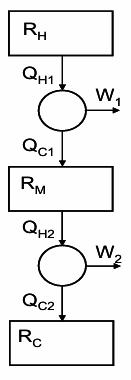
\includegraphics[width=0.14\textwidth]{images/3R-exemploentropia.png}
  \caption{Ilustração do Ciclo}
\end{wrapfigure}

Considerando três reservatórios de energia $R_H$, $R_M$ e $R_C$, e dois ciclos internamente reversíveis a operar entre estes: o primeiro ciclo opera entre os reservatórios $R_H$ e $R_M$, e o segundo entre os reservatórios $R_M$ e $R_C$. 

Os reservatórios, de volume constante, só trocam energia com as unidades de produção de trabalho dos ciclos e contêm a mesma massa do mesmo fluido incompressível com calor específico constante $c$.

Os reservatórios encontram-se inicialmente a $T_H$, $T_M$ e $T_C$, respetivamente. O sistema produz trabalho até os três reservatórios atingirem o equilíbrio térmico, onde as temperaturas dos reservatórios são igual a $T_f$.

\begin{eqnarray*}
    \Delta S = 0 \\
    \Delta S_H + \cancelto{0}{\Delta S_{ciclo_1}} + \Delta S_M + \cancelto{0}{\Delta S_{ciclo_2}} + \Delta S_C = 0 \\
    m c \ln \frac{T_f}{T_H} + m c \ln \frac{T_f}{T_M} + m c \ln \frac{T_f}{T_C} = 0 \\
    \ln \frac{T_f^3}{T_H T_M T_C} = 0 \\
    T_f = \sqrt[3]{T_H T_M T_C}
\end{eqnarray*}

Dado que o sistema produz trabalho, necessariamente: $T_H > T_M > T_C$, pelo que $T_C < T_f < T_H$, o que é um resultado correto: $T_H$ vai diminuindo fruto do calor cedido por $R_H$ ao ciclo, e $T_C$ vai aumentando e, portanto, a temperatura final terá de estar entres as duas temperaturas. 

O balanço de energia de todo o sistema dá:

\begin{eqnarray*}
    \Delta U = - W_1 - W_2 \\
    3 m c T_f - mc (T_H + T_M + T_C) = - W_T \\
    W_T =  mc \left[ (T_H + T_M + T_C) - 3 \sqrt[3]{T_H T_M T_C} \right] \\
\end{eqnarray*}

No entanto, se considerássemos que haveria irreversibilidades no sistema, obteríamos:

\begin{eqnarray*}
    \Delta S = \int \cancelto{0}{\frac{\delta Q}{T}} + \sigma \\
    m c \ln \frac{T_f^3}{T_H T_M T_C} = \sigma \\
    T_f = \sqrt[3]{T_H T_M T_C e^{\frac{\sigma}{m c}}}
\end{eqnarray*}

Assim, se $\sigma > 0$, $T_f \uparrow \implies W_T \downarrow$, e para $\sigma = 0$, obtemos $T_f = \sqrt[3]{T_H T_M T_C}$ ótimo, onde o trabalho total do sistema é máximo.

\end{examplebox}


\section{Trabalho em Sistemas Abertos}

O trabalho de um compressor ou uma turbina pode ser determinado da seguinte forma.

O balanço de energia, desprezando termos cinéticos e potenciais, dá:

\begin{eqnarray}
    \cancelto{0}{\frac{dE}{dt}} = \dot{Q} + \dot{W} + \dot{m} (h_1 - h_2) \\
    \frac{\dot{W}}{\dot{m}} = - \frac{\dot{Q}}{\dot{m}} + h_2 - h_1
\end{eqnarray}

O balanço de entropia dá, considerando a temperatura na fronteira do sistema constante:

\begin{eqnarray}
    \cancelto{0}{\frac{dS}{dt}} = \int \frac{\dot{q}}{T} + \dot{m} (s_1 - s_2) + \cancelto{0}{\dot{\sigma}}\\
    \frac{\dot{Q}}{T} = \dot{m} (s_2 - s_1) \\
    \frac{\dot{Q}}{\dot{m}} = T (s_2 - s_1)
\end{eqnarray}

De um modo geral, a temperatura pode variar, pelo que a expressão mais geral é:

\begin{equation}
    \left( \frac{\dot{Q}}{\dot{m}} \right)_{\substack{\text{int} \\ \text{rev}}} = \int_1^2 T ds
\end{equation}

onde o subscrito lembra-nos que a expressão é válida apenas para processos internamente reversíveis ($\sigma = 0$).

Assim, 
\begin{equation*}
    \frac{\dot{W}}{\dot{m}} = - \int_1^2 T ds + h_2 - h_1
\end{equation*}

De \ref{eq:2tds} ($ Tds = dh - v dp$), temos $-Tds + dh = v dp$, como $T=\text{const.}$, $\int -Tds + \int dh = \int v dp \Longleftrightarrow - \int T ds + \Delta h = \int v dp$.

Assim, obtemos o que pretendíamos

\begin{equation} \label{eq:w-intrev}
    \left( \frac{\dot{W}}{\dot{m}} \right)_{\substack{\text{int} \\ \text{rev}}} = \int_1^2 v dp
\end{equation}

onde o subscrito ``int. rev.'', indica que se refere ao trabalho total específico para um compressor/turbina internamente reversível. Localmente, pode-se dizer que as várias contribuições de trabalho $\delta W = - p dv$ resultam num trabalho global dado por esta expressão.

É de notar que a água, assim como outros líquidos considerados incompressíveis, com volume específico da ordem de grandeza $10^{-3}~\text{m}^3/\text{kg}$, aproximadamente constante, é muito mais fácil de comprimir, i.e. requer menos trabalho, do que um gás.
Considerando o ar gás ideal à temperatura e pressão ambiente, tem volume específico $v = \frac{RT}{p} = \frac{287 \cdot 298.15}{1\cdot 10^5} = 0.86~\text{m}^3/\text{kg}$, resultando num trabalho de compressão maior para a mesma pressão final.
Para o hidrogénio, $v = \frac{4124 \cdot 298.15}{1\cdot 10^5} = 12.3~\text{m}^3/\text{kg}$.

Assim, o trabalho específico para comprimir um kilograma de hidrogénio é muito maior do que um kilograma de água (1 kg de água ocupa $1~\text{L}$, enquanto 1 kg de hidrogénio $12000~\text{L}$). Quanto maior volume específico, maior o trabalho necessário para comprimir uma dada substância.

\subsection{Trabalho em Processos Politrópicos}

Para um processo politrópico $p v^n = c \implies v = \left(\frac{c}{p} \right)^{1/n}$:

\begin{itemize}
    \item Para $n \neq 1$:
    \begin{equation}
        \begin{split}
            \left( \frac{\dot{W}}{\dot{m}} \right)_{\substack{\text{int} \\ \text{rev}}} & = \int_{p_1}^{p_2} \left(\frac{c}{p} \right)^{1/n} \, dp  = c^{1/n} \frac{n}{n-1} \left(p_2^{1-1/n} - p_1^{1-1/n}\right)\\
            \left( \frac{\dot{W}}{\dot{m}} \right)_{\substack{\text{int} \\ \text{rev}}} & = \frac{n}{n-1} \left(p_2 v_2 - p_1 v_1\right), \quad n \neq 1
        \end{split}
    \end{equation}
    Para gás ideal:
    \begin{equation}
        \left( \frac{\dot{W}}{\dot{m}} \right)_{\substack{\text{int} \\ \text{rev}}} = \frac{n R}{n-1} \left(T_2 - T_1\right), \quad n \neq 1
    \end{equation}

    \item Para $n = 1$:
    \begin{equation}
        \begin{split}
            \left( \frac{\dot{W}}{\dot{m}} \right)_{\substack{\text{int} \\ \text{rev}}} & = \int_{p_1}^{p_2} \frac{c}{p} \, dp = c \ln \frac{p_2}{p_1}\\
            \left( \frac{\dot{W}}{\dot{m}} \right)_{\substack{\text{int} \\ \text{rev}}} & = p_1 v_1 \ln \frac{p_2}{p_1} = p_2 v_2 \ln \frac{p_2}{p_1}, \quad n = 1
        \end{split}
    \end{equation}
    Para gás ideal:
    \begin{equation}
        \left( \frac{\dot{W}}{\dot{m}} \right)_{\substack{\text{int} \\ \text{rev}}} = RT \ln \frac{p_2}{p_1}, \quad n = 1
    \end{equation}
\end{itemize}

\chapter{Ciclos}
\section{Tipos de Ciclos}

A eficiência avalia quão bem um sistema/ciclo converte a energia que é preciso fornecer ao sistema, indispensável para o seu funcionamento, no trabalho que se pretende obter, ou, no caso do rendimento de ciclos frigoríficos e bombas de calor, em quantidade de energia na forma de calor que se pretendia mover.

\begin{equation*}
    \eta = \frac{\text{``o que eu quero''}}{\text{``o que é preciso fornecer''}}
\end{equation*}

\subsection{Ciclo Motor}

Os ciclos motor têm como objetivo realizar trabalho, sendo preciso fornecer energia, normalmente sobre a forma de calor.
É preciso fornecer $Q_H$ para realizar $W_u$ e acabando inevitavelmente por ceder $Q_C$. Fazendo o balanço energético tem-se: $\Delta E = Q_H - W_u - Q_C$. Como se trata de um ciclo $\Delta E = 0$, pelo que $W_u = Q_H - Q_C$.

Portanto, a \textbf{eficiência térmica} de um ciclo motor é:

\begin{equation}
    \eta = \frac{W_u}{Q_H} = \frac{Q_H - Q_C}{Q_H}  = 1 - \frac{Q_C}{Q_H}
\end{equation}

onde $Q_H$ é a energia recebida pelo reservatório quente (combustível, radiação solar, reação nuclear controlada) e $Q_C$ a energia cedida ao reservatório frio. É claro que $Q_H > Q_C$ num ciclo motor, pois pretende-se que $W_u > 0$. Pela conservação da energia, a eficiência é $\eta \leq 1$. Se $Q_C = 0$, a eficiência térmica seria $100\%$, mas isto viola a Formulação de Kelvin-Planck. Assim, para o ciclo funcionar, parte do calor recebido $Q_H$ é obrigatoriamente transferido para a fonte fria, $Q_C$. Logo, $\eta < 1$, não havendo eficiências de $100\%$.
Esta conclusão pode ser considerado um \textbf{corolário da Segunda Lei da Termodinâmica}.

\subsubsection{Corolários de Carnot}

Outros dois corolários da Segunda Lei são conhecidos como Corolários de Carnot:

\begin{enumerate}
    \item A eficiência térmica de um processo irreversível é sempre menor que a eficiência térmica de um processo reversível, quando ambos operam entre os mesmos reservatórios.
    \item Todos os processos reversíveis a operar entre os mesmos dois reservatórios têm a mesma eficiência térmica.
\end{enumerate}

\begin{proof}
    Para demonstrar o primeiro corolário, basta considerar dois ciclos: um reversível R e o outro irreversível I a operar entre os mesmos dois reservatórios. Ambos recebem $Q_H$ e realizam trabalho $W_R$ e $W_I$. Pelo princípio da conservção da energia, ambos cedem calor ao reservatório frio igual a $Q_C = Q_H - W_R$ e $Q_C' = Q_H - W_I$. Considerando agora que o ciclo R opera no sentido contrário, e dado ser reversível as transferências de calor e trabalho mantém-se iguais, mas em sentido contrário. Desta forma, o reservatório quente mantém todas as suas propriedades, dado que recebe $Q_H$ de R e cede $Q_H$ a I. Assim, consideremos o sistema que engloba os dois ciclos e o reservatório quente, como cada parte deste sistema opera num ciclo ou não sofre alterações, então o sistema conjunto opera num ciclo. Além disso, este sistema troca calor com um único reservatório, pelo que, de acordo com Kelvin-Planck, $\oint \delta W > 0$, sendo irreversível, pois na sua operação pelo menos uma das suas partes é irreversível, o ciclo I. Desta forma, $W_R - W_I > 0 \Longleftrightarrow W_R > W_I$. Como ambos os ciclos inicialmente considerados recebem a mesma quantidade de energia, $Q_H$, $\eta_R > \eta_I$.
    O segundo corolário pode ser demosntrado igualmente para dois ciclos reversíveis. O ciclo conjunto é reversível, pelo que a igualdade de Kelvin-Planck é válida. Logo, $W_{R_1} = W_{R_2}$, e $\eta_{R_1}= \eta_{R_1}$ 
\end{proof}


\subsection{Ciclo Frigorífico e Bombas de Calor}

Nos ciclos frigoríficos ou bombas de calor, o sistema recebe $Q_C$ e $W_{\text{ciclo}}$, de modo a ceder $Q_H$, tal que $Q_H = Q_C + W_{\text{ciclo}}$, no caso ideal. Temos, então: $\Delta E = Q_C + W_{\text{ciclo}} - Q_H \implies W_{\text{ciclo}} = Q_H - Q_C$. Como é necessário fornecer trabalho $W_{\text{ciclo}} > 0$, então: $Q_H > Q_C$, novamente.

\subsubsection{Ciclo Frigorífico}

Um Ciclo Frigorífico tem como objetivo arrefecer um dado espaço. Por isso, o rendimento de um Ciclo Frigorífico, ou em inglês, \textit{coefficient of performance} (COP), é a razão entre o calor que se pretende remover da fonte fria (o frigorífico), e o trabalho que se teve de fornecer (e.g. energia elétrica).

\begin{equation}
    \text{COP}_{\text{frig.}} = \beta = \frac{Q_C}{W_{\text{ciclo}}} = \frac{Q_C}{Q_H - Q_C}
\end{equation}

\begin{equation}
    \beta = \frac{Q_C}{Q_H - Q_C} = \frac{Q_H - Q_H + Q_C}{Q_H - Q_C} = \frac{Q_H}{Q_H - Q_C} - 1 = \frac{1}{1 - \frac{Q_C}{Q_H}} - 1 = \frac{1}{\eta} - 1
\end{equation}

Assim, temos $\beta > 0$ e mostrámos que existe uma relação entre o rendimento do ciclo frigorífico e a eficiência do ciclo motor que se obtém invertendo a direção de operação do ciclo, entre os mesmos reservatórios.

\subsubsection{Bomba de Calor}

Na Bomba de Calor, o objetivo é transferir calor, $Q_H$, para um dado espaço, seja para manter uma habitação a uma temperatura superior à temperatura ambiente, seja em processos industriais. Por isso, o rendimento de uma Bomba de Calor é dado por:

\begin{equation}
    \text{COP}_{\text{bomba}} = \gamma = \frac{Q_H}{W_{\text{ciclo}}} = \frac{Q_H}{Q_H - Q_C}
\end{equation}

Se o trabalho que é necessário fornecer a uma Bomba de Calor (ou a um Ciclo Frigorífico), $W_{\text{ciclo}}$, aproximar-se de zero, o rendimento aproximar-se-ia de infinito. No entanto, se $W_{\text{ciclo}} = 0 \implies Q_H = Q_C$, pelo que o sistema iria tirar energia do reservatório frio e tranferi-la para o reservatório quente, espontaneamente -- pois nenhum trabalho foi fornecido --, o que viola a Formulação de Clausius.

Além disso, 

\begin{equation*}
    \gamma = \frac{Q_H}{Q_H - Q_C} = \frac{1}{1 - \frac{Q_C}{Q_H}}
\end{equation*}

pelo que $Q_H > Q_C \implies 0 < \frac{Q_C}{Q_H} < 1 \Longleftrightarrow 0 < 1 - \frac{Q_C}{Q_H} < 1 \implies \gamma > 1$.
Além disso, 

\begin{equation}
    \gamma = \frac{1}{\eta}
\end{equation}

i.e. o rendimento da Bomba de Calor é o inverso da eficiência do Ciclo Motor para o mesmo ciclo de processos a operar no sentido contrário entre os mesmos reservatórios. Caso a Bomba de Calor seja reversível, o seu rendimento é igual ao rendimento de qualquer outra Bomba de Calor reversível a operar entre os mesmos reservatórios e maior do que o rendimento de qualquer ciclo irreversível a operar entre os mesmos reservatórios.

Assim, os Corolários de Carnot também são válidos para os ciclos frigoríficos e bombas de calor, bastando, para isso, substituir o termo \textit{eficiência térmica} por \textit{rendimento}.


\subsection{Escala de Kelvin}

Do segundo corolário de Carnot, sabemos que quaisquer dois ciclos a operar entre os mesmos dois reservatórios têm a mesma eficiência térmica, sendo, portanto, independente dos processos internos de cada ciclo. Portanto, a eficiência térmica está apenas relacionada com a natureza dos reservatórios. Como é a diferença de temperatura que permite as trocas de calor e a produção de trabalho, concluimos que a eficiência térmica depende apenas das temperaturas dos reservatórios.

\begin{equation}
    \left( \frac{Q_C}{Q_H} \right)_{rev} = f(T_C, T_H)
\end{equation}

Esta equação pode ser usada como base para definir uma escala de temperatura, independente das propriedades da substância. A Escala de Kelvin foi definida então para $f = \frac{T_C}{T_H}$: 

\begin{equation}
    \left( \frac{Q_C}{Q_H} \right)_{rev} = \frac{T_C}{T_H}
\end{equation}

Assim, se um ciclo operar entre um reservatório a $273.16 K$ (temperatura do ponto triplo da água) e outra a uma temperatura $T$,

\begin{equation*}
    T = 273.16 \left( \frac{Q}{Q_{pt}} \right)_{rev}
\end{equation*}

Desta forma, quando $Q \to 0$, também $T \to 0$, pelo que podemos concluir que o zero absoluto é a menor temperatura atingível na Escala de Kelvin, ou escala absoluta de temperatura.

\subsection{Eficiência de Carnot}

\subsubsection{Ciclo Motor}

\begin{equation}
    \eta_{max} = 1 - \frac{T_C}{T_H}
\end{equation}

Note-se que a eficiência aumenta com $T_H$ mais elevada e/ou $T_C$ mais baixa. No entanto, em ciclos motores, a redução de $T_C$ é geralmente limitada por restrições práticas, uma vez que temperaturas inferiores à ambiente requerem um sistema frigorífico.

Estas conclusões estão qualitativamente corretas para ciclos reais, irreversíveis. Muitas vezes, maximizar a eficiência térmica pode não ser o único objetivo. Considerações de custo e limitações físicas podem mostrar que uma eficiência de 40 \% pode não parecer assim tão pouco, relativamente a um valor limitante realista de 60\%, por exemplo, em vez de 100\%.

\subsubsection{Ciclo Frigorífico}

\begin{equation}
    \beta_{max} = \frac{T_C}{T_H - T_C}
\end{equation}

\subsubsection{Bomba de Calor}

\begin{equation}
    \gamma_{max} = \frac{T_H}{T_H - T_C}
\end{equation}

Note-se que as temperaturas têm de ser temperaturas absolutas na escala de Kelvin ou na de Rankine, pois são escalas absolutas que diferem de um fator multiplicativo: $T(\text{\textdegree R}) = 1.8 \, T(\text{K})$, enquanto as escalas de Celsius e Fahrenheit têm uma translação arbitrária em relação ao zero absoluto.


\subsection{Ciclo de Carnot}

Num Ciclo de Carnot, um sistema passa por quatro processos internamente reversíveis: dois \textbf{processos adiabáticos} alternados com dois \textbf{processos isotérmicos}.

Exemplo do Ciclo de Carnot para um sistema de gás num êmbolo-cilindro. As paredes do sistema são adiabáticas.

\begin{itemize}
    \item \textbf{Processo 1 $\rightarrow$ 2:} O sistema entra em contacto com o reservatório a $T_H$. O gás expande isotermicamente, enquanto recebe $Q_H$.
    \item \textbf{Processo 2 $\rightarrow$ 3:} O gás é permitido expandir adiabaticamente até a temperatura diminuir até $T_C$.
    \item \textbf{Processo 3 $\rightarrow$ 4:} O sistema entra em contacto com o reservatório a $T_C$. O gás comprime isotermicamente, cedendo $Q_C$.
    \item \textbf{Processo 4 $\rightarrow$ 1:} O gás é comprimido adiabaticamente até atingir $T_H$.
\end{itemize}

Para o Processo 1 $\rightarrow$ 2 ser reversível, a diferença entre a temperatura do gás e a temperatura do reservatório deve ser tendencionalmente nula. Desta forma, dado que o reservatório mantém a sua temperatura, implica que a temperatura do gás também deve ser constante. Idem, para o Processo 3 $\rightarrow$ 4.

Um Ciclo de Carnot a operar na direção contrária é um Ciclo Frigorífico ou uma Bomba de Calor. Um Ciclo de Carnot também pode ser composto por processos onde um condensador é carregado e descarregado, ou uma substância paramagnética é magnetizada ou desmagnetizada.

\subsubsection{Trabalho Compressão/Expansão}

Para um gás ideal, num sistema êmbolo-cilindro como descrito anteriormente, sabemos que o trabalho dos processos de compressão e expansão isotérmicos é dado por \ref{eq:trabalho-gas-ideal}:

\begin{equation}
    W = - mRT \ln \frac{V_2}{V_1} = - mRT \ln \frac{\frac{mR T}{p_2}}{\frac{mR T}{p_1}} = - mRT \ln \frac{p_1}{p_2} = mRT \ln \frac{p_2}{p_1}
\end{equation}

E, assim, podemos observar, no Ciclo de Carnot, que:

\begin{itemize}
    \item \textbf{Compressão ($p_2 > p_1$)}: é necessário arrefecer (ceder $Q_C$ no Processo 3 $\rightarrow$ 4) o sistema para diminuir a entropia e para diminuir o trabalho de compressão, pois $T \downarrow \implies W \downarrow$.
    \item \textbf{Expansão ($p_2 < p_1$)}: no Processo 1 $\rightarrow$ 2, pretende-se obter o máximo de calor, $Q_H$, para aumentar a temperatura do sistema, pois, quanto maior a temperatura, maior será o trabalho obtido na expansão ($T \uparrow \implies W \uparrow$).
\end{itemize}



\section{Ciclo de Carnot}

O Ciclo de Carnot pode ser aplicado a um um ciclo motor reversível com água circulante, onde $\nabla T, \nabla P \to 0$ e $\sigma = 0$, considerando \textbf{processos adiabáticos} na turbina e na bomba, e \textbf{processos isotérmicos} no condensador e na caldeira.

\begin{itemize}
    \item \textbf{Processo 1 $\rightarrow$ 2 (Caldeira):} A água passa do estado líquido ao gasoso isotermicamente, logo, a pressão constante, enquanto recebe $Q_H$.
    \item \textbf{Processo 2 $\rightarrow$ 3 (Turbina):} O vapor, que sai da caldeira, expande na turbina adiabaticamente, realizando trabalho. A temperatura diminui para $T_C$ e a pressão diminui.
    \item \textbf{Processo 3 $\rightarrow$ 4 (Condensador):} Algum vapor condensa isotermicamente a $T_C$, a pressão constante.
    \item \textbf{Processo 4 $\rightarrow$ 1 (Bomba):} A bomba recebe a mistura de duas fases do condensador e comprime adiabaticamente até $T_H$. 
\end{itemize}

\begin{figure}[H]
    \centering
    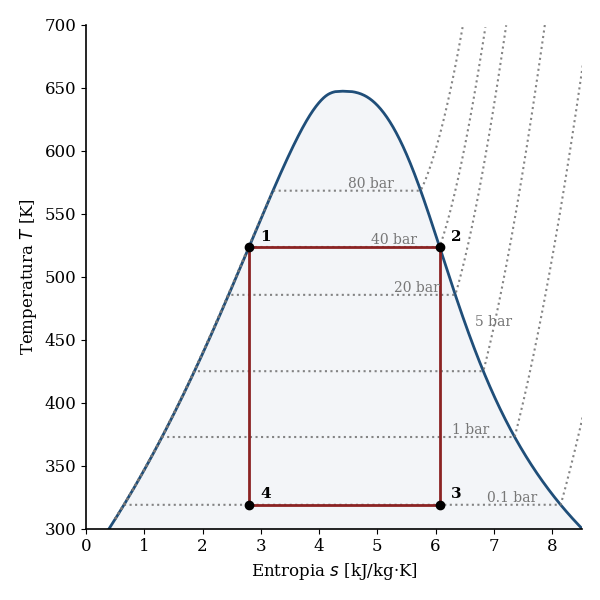
\includegraphics[width=0.45\linewidth]{graphs/carnot-Ts-ideal.png}
    \caption{Ciclo Carnot}
    \label{fig:carnot-Ts}
\end{figure}

Como se tratam de processos reversíveis, no contacto com os reservatórios: $ds = \frac{\delta Q}{T} + \delta \cancelto{0}{\sigma}$ e temos, então $\delta Q = T ds$. Logo, o valor do integral: $Q = \int T ds$, é igual ao calor total transferido no contacto com os reservatórios. Num diagrama T-s, este corresponde à área por baixo das linhas isotérmicas $T_H$ e $T_C$.

Fazendo os balanços de energia e entropia para cada processo, obtém-se:

\begin{itemize}
    \item \textbf{Processo 1 $\rightarrow$ 2 (Caldeira):} $\Delta U_{12} = Q_H - W_{12}$ e $\Delta S_{12} = \frac{Q_{H}}{T_H}$
    \item \textbf{Processo 2 $\rightarrow$ 3 (Turbina):} $\Delta U_{23} = -W_{23}$ e $\Delta S_{23} = 0$
    \item \textbf{Processo 3 $\rightarrow$ 4 (Condensador):} $\Delta U_{34} = -Q_C + W_{34}$ e $\Delta S_{34} = - \frac{Q_{C}}{T_C}$
    \item \textbf{Processo 4 $\rightarrow$ 1 (Bomba):} $\Delta U_{41} = W_{41}$ e $\Delta S_{41} = 0$
\end{itemize}

Como se trata de um ciclo $\Delta U = 0$, então:
\begin{equation*}
    \sum_i \Delta U_i = \sum_i Q_i + \sum_i W_i \Longleftrightarrow 0 = Q_H - Q_C - W_{12} - W_{23} + W_{34} + W_{41}
\end{equation*}

Portanto, o trabalho útil do ciclo é:

\begin{equation}
    W_u = W_{12} + W_{23} - ( W_{34} +  W_{41}) = Q_H - Q_C
\end{equation}

Ou, de outra forma, o trabalho do ciclo é $W_u = \int T_H ds + \int T_C ds = T_H \Delta S_{12} +  T_C \Delta S_{34} = Q_H - Q_C$.


No ciclo, $\sum_i \Delta S_i = 0 \Longleftrightarrow \Delta S_{12} + \Delta S_{34} = 0 \Longleftrightarrow \frac{Q_H}{T_H} - \frac{Q_C}{T_C} = 0 \implies \frac{Q_C}{Q_H} = \frac{T_C}{T_H}$. E, novamente,

\begin{equation}
    \eta_{rev} = 1 - \frac{Q_C}{Q_H} = 1 - \frac{T_C}{T_H}
\end{equation}

\begin{examplebox}[Ciclos Reversíveis]

O trabalho do ciclo $W_u = \int T_H ds + \int T_C ds $ pode ser generalizado para qualquer ciclo reversível, onde o trabalho útil do ciclo será a área contida entre as linhas dos processos do ciclo.

\begin{figure}[H]
    \centering
    \begin{subfigure}{0.32\textwidth}
        \centering
        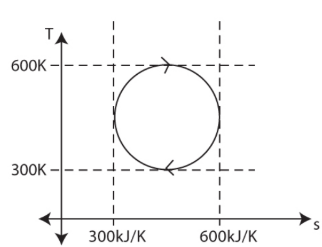
\includegraphics[width=\textwidth]{images/ciclo-circulo.png}
        \caption{Ciclo reversível - círculo}
        \label{fig:rev-circulo}
    \end{subfigure}
    \hfill
    \begin{subfigure}{0.62\textwidth}
        \centering
        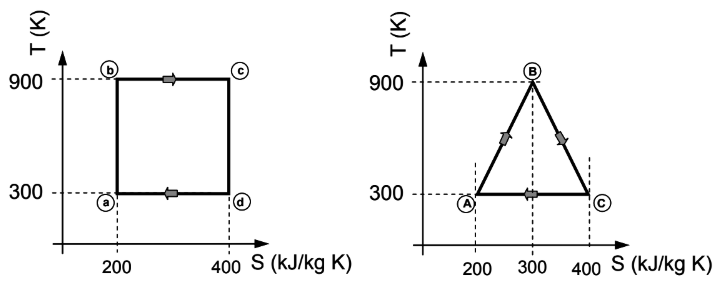
\includegraphics[width=\textwidth]{images/ciclos-triangulo.png}
        \caption{Quadrado (Carnot) e Triângulo}
        \label{fig:rev-triangulo}
    \end{subfigure}
    \caption{Exemplos de ciclos reversíveis}
\end{figure}

\begin{itemize}
    \item Círculo: $W_u = \text{``área do círculo''} = \pi \cdot 150^2$ (kJ)
    \item Quadrado: $W_u = T_H \Delta S_{bc} + T_C \Delta S_{da} = 900\cdot(400-200) + 300\cdot (200 -400) = 120000~\text{kJ/kg}$\\
                    ou $W_u = \text{``área do quadrado''} = (900 - 300)\cdot(400-200)= 120000~\text{kJ/kg}$
    \item Triângulo: $W_u = (400-200) \cdot (900 -300) /2 = 60000~\text{kJ/kg}$
\end{itemize}

\end{examplebox}


\subsection{Ciclo Motor Real}

Num ciclo real, quando o sistema entra em contacto com o reservatório a $T_H$, o sistema está a $T_H' < T_H$, e, quando entra em contacto com o reservatório a $T_C$, encontra-se a $T_C' > T_C$, tal como representado na Figura \ref{fig:ciclo-real}.

\begin{figure}[H]
    \centering
    \begin{tikzpicture}[scale=1.1, every node/.style={font=\small}]
        % Heat reservoirs
        \node[draw, minimum width=3cm, minimum height=0.8cm, fill=red!10] (TH) at (0,3.4) {Fonte Quente ($T_H$)};
        \node[draw, minimum width=3cm, minimum height=0.8cm, fill=blue!10] (TC) at (0,0) {Fonte Fria ($T_C$)};
        
        % Heat engine
        \node[draw, minimum width=3cm, minimum height=1.5cm, fill=gray!10] (engine) at (0,1.7) {Máquina térmica real};

        % Arrows
        \draw[->, thick] (TH.south) -- node[right] {$T_H' < T_H$} (engine.north);
        \draw[->, thick] (engine.south) -- node[right] {$T_C' > T_C$} (TC.north);

        % Entropy labels
        \node at (2.3,2.7) {$\sigma_f$};
        \node at (2.3,1.7) {$\sigma_m$};
        \node at (2.3,0.7) {$\sigma_f$};

        % System boundaries
        \draw[dashed, thick, red!60] (-2,3.1) rectangle (2,0.3);
        \node[red!60] at (4.43,3.2) {\footnotesize Fronteira infinitesimal ($\sigma_m + \sigma_f$)};

        \draw[dashed, thick, blue!60] (-2,2.3) rectangle (2,1.1);
        \node[blue!60] at (-4,2) {\footnotesize Fronteira do motor ($\sigma_m$)};
    \end{tikzpicture}
    \caption{Representação esquemática de um ciclo térmico real e as fontes de irreversibilidades.}
    \label{fig:ciclo-real}
\end{figure}

Assim, considerando um sistema que engloba uma parte infinitesimal dos reservatórios para lá da fronteira entre o ciclo interno e os reservatórios, e tendo $\Delta S = 0$ para um ciclo, o balanço de entropia dá:

\begin{equation*}
    \cancelto{0}{\Delta S} = \frac{Q_H}{T_H} - \frac{Q_C}{T_C} + \sigma_{motor} + \sigma_{fronteira} \implies Q_C = \frac{T_C}{T_H} Q_H + T_C (\sigma_m +\sigma_f)
\end{equation*}

\begin{equation*}
    W_u = Q_H - Q_C = Q_H - \frac{T_C}{T_H} Q_H - T_C (\sigma_m +\sigma_f) = Q_H \left(1 - \frac{T_C}{T_H} \right) - T_C(\sigma_m +\sigma_f)
\end{equation*}

\begin{equation} \label{eq:eta-fronteira}
    \eta = \frac{W_U}{Q_H} = \eta_{rev} - \frac{T_C}{Q_H}(\sigma_m +\sigma_f)
\end{equation}

Por outro lado, considerando um sistema imediatamente antes da fronteira do ciclo interno com os reservatórios, o balanço de entropia do ciclo não terá em conta irreversibilidades associadas às trocas de calor pela fronteira:

\begin{equation*}
    \cancelto{0}{\Delta S} = \frac{Q_H}{T_H'} - \frac{Q_C}{T_C'} + \sigma_{m} \implies Q_C = \frac{T_C'}{T_H'} Q_H + T_C' \sigma_m
\end{equation*}

\begin{equation*}
    W_u = Q_H \left(1 - \frac{T_C'}{T_H'} \right) - T_C' \sigma_m
\end{equation*}

\begin{equation} \label{eq:antes-fronteira}
    \eta = \frac{W_U}{Q_H} = 1 - \frac{T_C'}{T_H'} - \frac{T_C'}{Q_H} \sigma_m
\end{equation}

Podemos obter estimativas experimentais para os termos de geração de entropia \( \sigma_m \) e \( \sigma_f \), utilizando as temperaturas efetivas de troca térmica (\( T_H' \), \( T_C' \)) e os calores \( Q_H \) e \( Q_C \) medidos. A partir da equação \ref{eq:antes-fronteira}, pode-se isolar \( \sigma_m \), e, substituindo o resultado na equação \ref{eq:eta-fronteira}, é possível determinar \( \sigma_f \):

\begin{equation}
    \sigma_m = \frac{Q_C - \frac{T_C'}{T_H'} Q_H}{T_C'} \qquad \text{e} \qquad \sigma_f = \frac{Q_C - \frac{T_C}{T_H} Q_H}{T_C} - \sigma_m
\end{equation}

Esta abordagem permite distinguir os efeitos das irreversibilidades internas ao ciclo térmico (\( \sigma_m \)), como atritos, dissipações ou choques térmicos, daqueles associados às trocas de calor com os reservatórios (\( \sigma_f \)), resultantes da existência de gradientes finitos de temperatura.



\section{Ciclo de Rankine}

O Ciclo de Rankine surge de forma a adaptar o Ciclo de Carnot às limitações da engenharia real. A presença de vapor de água no estágio de compressão não é benéfico para a bomba, causando desgaste e aumentando o trabalho necessário para comprimir. O Ciclo de Rankine resolve essa limitação ao garantir que a compressão ($1 \rightarrow 2$) ocorra com o fluido completamente no estado líquido.

Tal como no Ciclo de Carnot, o Ciclo de Rankine Ideal considera a compresão na bomba e a expansão na turbina como \textbf{processos adiabáticos}. Perdas de energia por transferências de calor entre os componentes e variações na energia cinética e pontencial são desprezadas.

\begin{figure}[H]
    \centering
    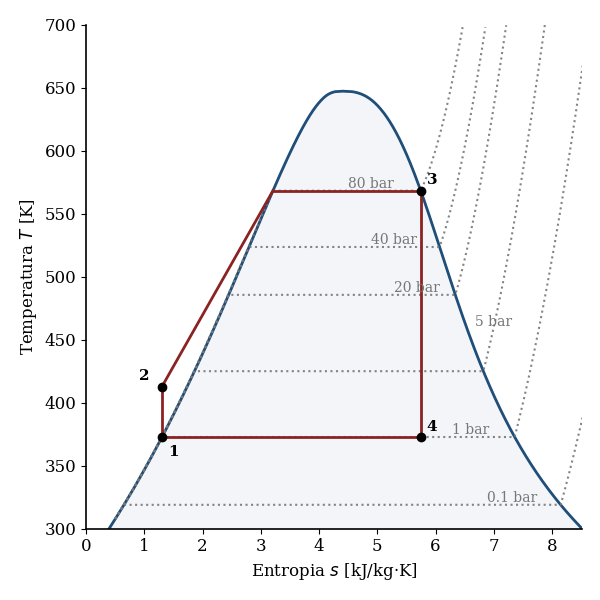
\includegraphics[width=0.45\linewidth]{graphs/rankine-Ts-ideal-ideal.png}
    \caption{Ciclo de Rankine Ideal}
    \label{fig:rankine-Ts-ideal-ideal}
\end{figure}

\subsection{Ciclo de Rankine Sobreaquecido}

De forma semelhante à compressão, durante a expansão na turbina a presença de gotas de água diminui a eficiência da turbina e aumenta a necessidade de manutenção da turbina, pelo que é comum manter a qualidade na saída da turbina ser de pelo menos $90 \%$.

Por outro lado, estamos a aumentar a temperatura média de adição de calor $\bar{T}_H$, pelo que a eficiência térmica do ciclo aumenta.

Para isso, é necessário aquecer mais a água, aumentando $T_3$. É de notar que aumentando a temperatura também aumenta $v$, pelo que o trabalho gerado na turbina será maior. De igual forma, sendo as isobáricas divergentes, o rácio $\frac{Q_C}{Q_H}$ diminui, aumentando a eficiência do ciclo.

Assim, de um ponto de vista teórico, o ideal seria que o fluido saísse da turbina com título $x=1$, i.e. vapor saturado, tal como na Figura \ref{fig:rankine-Ts-ideal-sobreaquecido}, havendo menor condensação e menor erosão mecânica das pás por impacto de gotículas de água. No entanto, na engenharia prática, tal não é viável.

\begin{figure}[H]
    \centering
    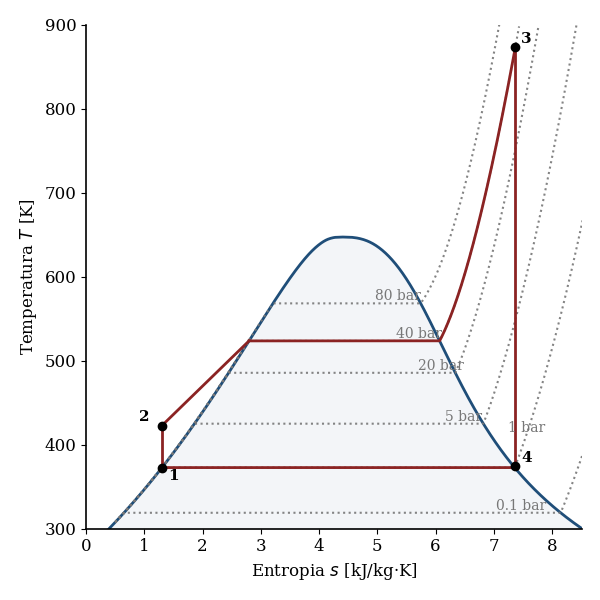
\includegraphics[width=0.45\textwidth]{graphs/rankine-Ts-ideal-sobreaquecido.png}
    \caption{Ciclo de Rankine Sobreaquecido}
    \label{fig:rankine-Ts-ideal-sobreaquecido}
\end{figure}

Um exemplo de um Ciclo de Rankine é uma central de produção de energia elétrica, representada na Figura \ref{fig:rankine-Ts-ideal-powerplant}, que trabalha entre $0.1~\text{bar}$ e $80~\text{bar}$ com uma temperatura máxima de $773.15~\text{K}$ e $319~\text{K}$ de mínima: 

\begin{figure}[H]
    \centering
    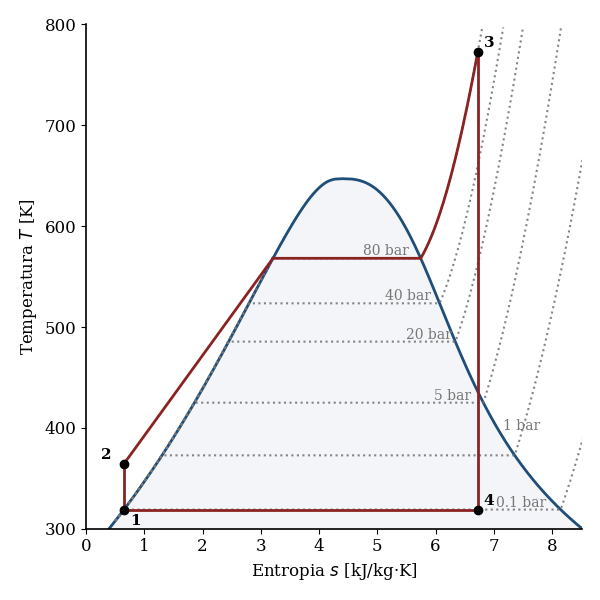
\includegraphics[width=0.45\linewidth]{graphs/rankine-Ts-ideal-powerplant.png}
    \caption{Ciclo de Rankine de uma Central Elétrica}
    \label{fig:rankine-Ts-ideal-powerplant}
\end{figure}

Na verdade, o estado 2, após a compressão na bomba está exagerado, dado que, em condições ideais, a temperatura da água aumentaria apenas cerca de $0.268~\text{K}$. O gráfico à escala está representado na Figura \ref{fig:rankine-Ts-ideal-true-powerplant}. Na Figura \ref{fig:rankine-pump-amp}, pode-se observar a proximidade das isobáricas à curva da água líquida saturada. Esta proximidade evidencia a facilidade (baixo trabalho) em comprimir água líquida, devido ao baixo volume específico. Recordando $(\frac{\dot{W}}{\dot{m}} = \int v dp)$

\begin{figure}[H]
    \centering
    \begin{subfigure}{0.45\textwidth}
        \centering
        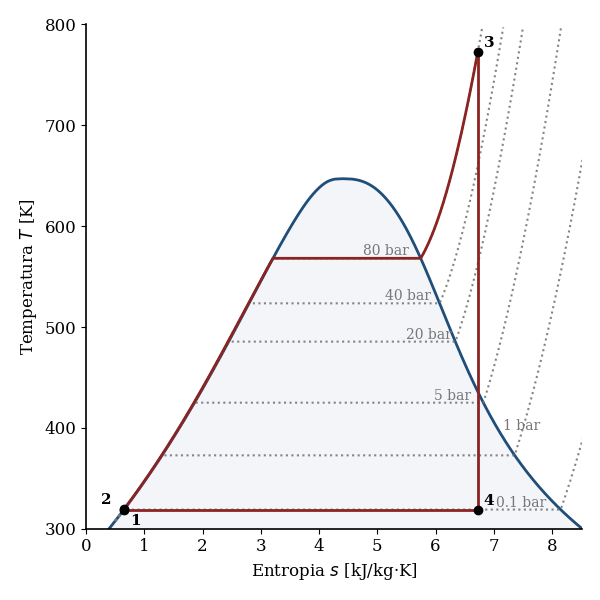
\includegraphics[width=\textwidth]{graphs/rankine-Ts-ideal-true-powerplant.png}
        \caption{Ciclo de Rankine à escala}
        \label{fig:rankine-Ts-ideal-true-powerplant}
    \end{subfigure}
    \hfill
    \begin{subfigure}{0.4\textwidth}
        \centering
        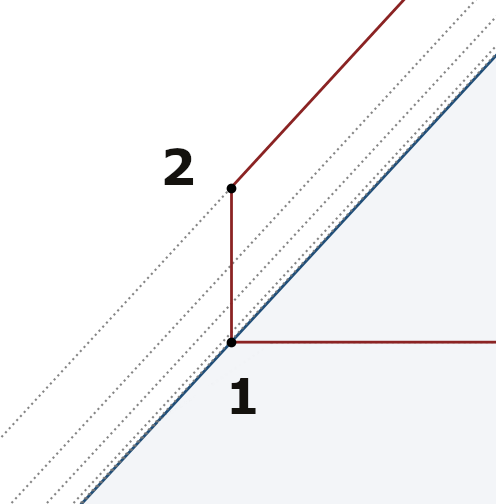
\includegraphics[width=\textwidth]{graphs/pump-amp.png}
        \caption{Ampliação do Processo de Compressão}
        \label{fig:rankine-pump-amp}
    \end{subfigure}
    \caption{Compressão à escala real}
\end{figure}

Considerando cada componente que compõe o ciclo isoladamente e aplicando o balanço de energia, podemos obter o trabalho e o calor específicos de cada componente.

Pode-se notar que o módulo destas quantidades é sempre dado pela diferença de entalpia entre o ponto onde o fluido circulante tem maior entalpia e o ponto onde esta é menor. Por exemplo, na bomba o fluido terá mais energia (entalpia) após a compressão, logo, considerando a compressão um processo adiabático:

\begin{eqnarray*}
    \cancelto{0}{\frac{dE}{dt}} = \cancelto{0}{\dot{Q}} + \dot{W_b} + \dot{m} (h_1 - h_2) \\
    \frac{\dot{W}_b}{\dot{m}} = h_2 - h_1
\end{eqnarray*}

\begin{itemize}
    \item \textbf{Processo 1 $\rightarrow$ 2 (Bomba):} $\frac{\dot{W}_b}{\dot{m}} = h_2 - h_1$
    \item \textbf{Processo 2 $\rightarrow$ 3 (Caldeira):} $\frac{\dot{Q}_H}{\dot{m}} = h_3 - h_2$
    \item \textbf{Processo 3 $\rightarrow$ 4 (Turbina):} $\frac{\dot{W}_t}{\dot{m}} = h_3 - h_4$
    \item \textbf{Processo 4 $\rightarrow$ 1 (Condensador):} $\frac{\dot{Q}_C}{\dot{m}} = h_4 - h_1$
\end{itemize}

No caso da bomba, sendo água líquida, também podemos calcular o trabalho para um processo internamente reversível, por (tal como visto em \ref{eq:w-intrev}):

\begin{equation}
    \left( \frac{\dot{W}_b}{\dot{m}} \right)_{\substack{\text{int} \\ \text{rev}}} = \int v dp \approx v (p_2 - p_1)
\end{equation}

que é, na verdade, a mesma expressão, pois processos internamente reversíveis e adiabáticos (que são as condições, tanto na bomba, como na turbina no ciclo de Rankine ideal) são isentrópicos, e da Equação \ref{eq:2tds} (válida para processos internamente reversíveis) temos: $dh = \cancelto{0}{Tds} + vdp \implies dh = vdp$.

\subsection{Ciclo de Rankine Real}

Considerando que a bomba e a turbina não são ideais, obtemos uma representação de um ciclo real, como a da Figura \ref{fig:rankine-Ts-real-powerplant}, sem considerar perdas de pressão nas tubagens.

\begin{figure}[H]
    \centering
    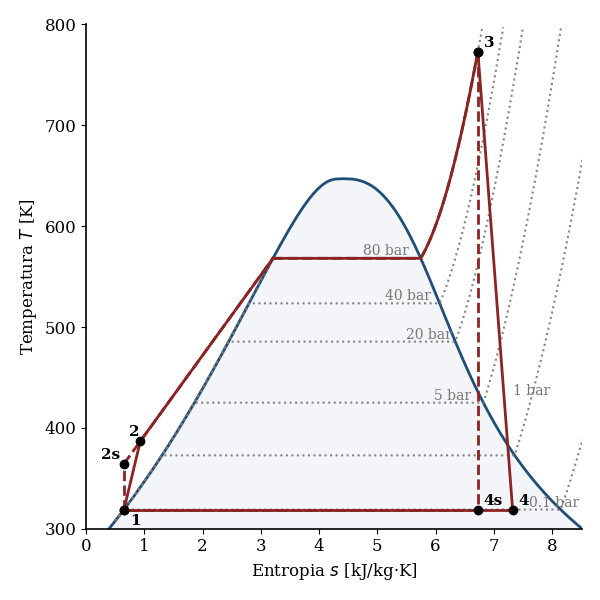
\includegraphics[width=0.45\linewidth]{graphs/rankine-Ts-real-powerplant.png}
    \caption{Ciclo de Rankine Real}
    \label{fig:rankine-Ts-real-powerplant}
\end{figure}

Pode-se pensar que, na bomba, o ideal é fornecer o menor trabalho possível que na mesma atinja o objetivo. Desta forma, o trabalho isentrópico (sem irreversibilidades) será menor que o trabalho real, onde se gera entropia.

Por isso, a \textbf{eficiência isentrópica} do compressor é dada por:

\begin{equation}
    \eta_b = \frac{(\dot{W}_b/\dot{m})_s}{(\dot{W}_b/\dot{m})} = \frac{h_{2s} - h_1}{h_{2} - h_1}
\end{equation}

Por outro lado, na turbina o caso ideal é quando recebemos o maior trabalho possível e, portanto, o trabalho isentrópico será maior que o trabalho real:

\begin{equation}
    \eta_t = \frac{(\dot{W}_t/\dot{m})}{(\dot{W}_t/\dot{m})_s} = \frac{h_3 - h_4}{h_3 - h_{4s}}
\end{equation}

Como o trabalho da bomba é muito menor que o trabalho da turbina, as irreversibilidades na bomba têm normalmente um impacto menor na eficiência térmica do que as da turbina. A maior fonte de irreversibilidade está associada à combustão e a transferência de calor dos produtos de combustão para o fluido circulante.

A eficiência do ciclo de Rankine é:

\begin{equation}
    \eta = \frac{W_t - W_c}{Q_H} = \frac{h_3 - h_4 - (h_2 - h_1)}{h_3 - h_2} = 1 - \frac{h_4 - h_1}{h_3 - h_2} = 1 - \frac{T_4 - T_1}{T_3 - T_2} 
\end{equation}

Comparando com a eficiência máxima de Carnot:

\begin{equation*}
    \eta = \frac{Q_H - Q_c}{Q_H} = 1 - \frac{Q_c}{Q_H} = 1 - \frac{\frac{\dot{Q}_C}{\dot{m}}}{\frac{\dot{Q}_H}{\dot{m}}} = 1 -\frac{T_C (s_{4s} - s_1)}{\bar{T}_H (s_3 - s_{2s})} = 1 -\frac{T_C}{\bar{T}_H}
\end{equation*}

Como a temperatura média $\bar{T}_H$ de adição de calor na fonte quente é inferior a $T_H$, o ciclo de Rankine ideal tem uma eficiência menor que o ciclo de Carnot ideal entre as mesmas fontes. Assim, a eficiência do ciclo tende a aumentar com o aumento de $\bar{T}_H$ e/ou a diminuição de $\bar{T}_C$.



\section{Ciclo de Brayton}

O Ciclo de Brayton faz parte de ciclo de turbinas a gás. Considera-se como fluido circulante do ciclo ar como gás perfeito. Na expansão isotérmica de 4 para 1, não está conectado, pois muitas vezes o ar é expelido para a atmosfera em 4 na mesma pressão e a uma temperatura superior à de entrada em 1.

O ciclo opera entre duas pressões: a de entrada e saída, $p_1$, e a pressão de trabalho $p_2$ ($p_2 > p_1$). A razão de pressão é definida como: $r_p = \frac{p_2}{p_1} = \frac{p_3}{p_4}$.

Normalmente, é sabido $p_1$, $T_1$, ambiente, e $T_3$, após a combustão e condicionado por limitações físicas dos materiais das turbinas.

Para gás perfeito temos $\Delta s = c_p \ln \frac{T}{T_0} - R \ln \frac{p}{p_0}$, pelo que as isobáricas são exponenciais: $T = T_0 e^{\frac{\Delta s + R \ln \frac{p}{p_0}}{c_p}}$

\begin{figure}[H]
    \centering
    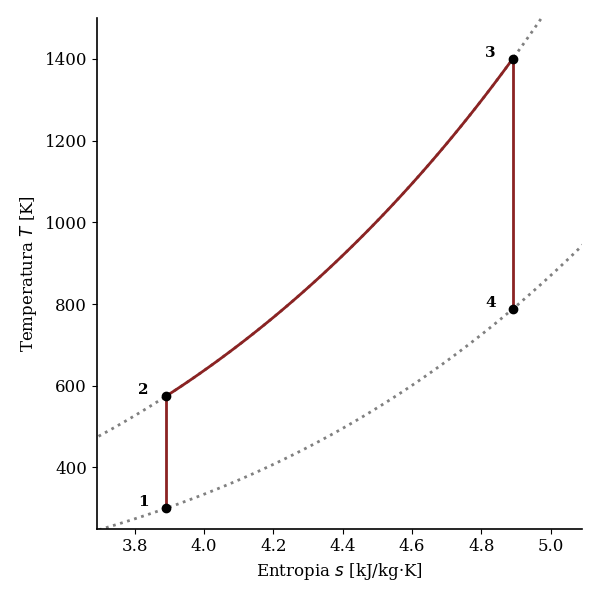
\includegraphics[width=0.45\linewidth]{graphs/brayton-Ts-ideal.png}
    \caption{Ciclo de Brayton Ideal}
    \label{fig:brayton-Ts-ideal}
\end{figure}

\begin{itemize}
    \item \textbf{Processo 1 $\rightarrow$ 2 (Compressor):} $\frac{\dot{W}_c}{\dot{m}} = h_2 - h_1$
    \item \textbf{Processo 2 $\rightarrow$ 3 (Combustão):} $\frac{\dot{Q}_H}{\dot{m}} = h_3 - h_2$
    \item \textbf{Processo 3 $\rightarrow$ 4 (Turbina):} $\frac{\dot{W}_t}{\dot{m}} = h_3 - h_4$
\end{itemize}

Neste exemplo, $T_1 = 300~\text{K}$, $T_3 = 1400~\text{K}$ e $p_1 = 1~\text{bar}$, $r_p = 10$, pelo que $p_2 = 10~\text{bar}$.

Como são processos isentrópicos $\frac{T_2}{T_1} = \left( \frac{p_2}{p_1} \right)^{(k-1)/k}$, podemos obter as temperaturas:

\begin{eqnarray}
    T_2 = T_1 \left( \frac{p_2}{p_1} \right)^{(k-1)/k} = T_1 \left( r_p \right)^{(k-1)/k} \\
    T_4 = T_3 \left( \frac{p_4}{p_3} \right)^{(k-1)/k} = T_3 \left( \frac{1}{r_p} \right)^{(k-1)/k}
\end{eqnarray}

A eficiência do Ciclo de Brayton é:

\begin{equation*}
    \eta = \frac{W_t - W_c}{Q_H} = \frac{h_3 - h_4 - (h_2 - h_1)}{h_3 - h_2} = 1 - \frac{h_4 - h_1}{h_3 - h_2} = 1 - \frac{T_4 - T_1}{T_3 - T_2} = 1 - \frac{T_1 \left(\frac{T_4}{T_1} -1\right)}{T_2 \left(\frac{T_3}{T_2} -1\right)}
\end{equation*}

Como

\begin{equation*}
    r_p = \frac{p_2}{p_1} = \frac{p_3}{p_4} \implies \frac{T_2}{T_1} = \frac{T_3}{T_4} \implies \frac{T_4}{T_1} = \frac{T_3}{T_2}
\end{equation*}

concluimos, então, que a eficiência do ciclo é:

\begin{equation}
    \eta = 1 - \frac{T_1}{T_2} = 1 - \left(\frac{1}{r_p}\right)^{(k-1)/k}
\end{equation}

Esta é a eficiência máxima de um Ciclo de Brayton real, substituindo $T_2$ por $T_{2s}$. A eficiência real do ciclo tem de ser calculado por $\eta = \frac{W_t - W_c}{Q_H} = 1 - \frac{h_4 - h_1}{h_3 - h_2} = 1 - \frac{T_4 - T_1}{T_3 - T_2}$. 

Podemos ver que a eficiência no Ciclo de Brayton Ideal, a eficiência do ciclo depende somente da razão de pressão e, por isso, do estágio de compressão. Quanto maior a razão de pressão, maior a eficiência.

\subsection{Trabalho máximo}

Podemos ver qual a razão de pressão ótima, tal que o trabalho útil é máximo.

A razão de pressão é máxima quando aumentamos $p_2 \to p_{max}$, no limite só podemos aumentar esta até que $T_2 \to T_3$, pelo que $r_{p_{max}} = \frac{p_{max}}{p_1} = \left(\frac{T_3}{T_1}\right)^{k/(k-1)}$

O trabalho útil é:

\begin{equation*}
    \dot{W}_u = \dot{W}_t - \dot{W}_c = h_3 - h_4 - (h_2 - h_1) = \dot{m} c_p (T_3 - T_4) - \dot{m} c_p (T_2 - T_1)
\end{equation*}

Dividindo para obter o trabalho específico e simplificar os cálculos:

\begin{equation*}
\begin{split}
    \frac{\dot{W}_u}{\dot{m} c_p T_1} & = \frac{T_3}{T_1} \left(1 - \frac{T_4}{T_3}\right) - \left(\frac{T_2}{T_1}-1\right)\\
    & = (r_{p_{max}})^{(k-1)/k} \left(1 - \left(\frac{1}{r_p}\right)^{(k-1)/k}\right) - \left((r_p)^{(k-1)/k} -1 \right)
\end{split}
\end{equation*}

Para encontrar o máximo, derivamos e igualamos a zero para encontraro ponto de máximo:

\begin{equation*}
\begin{split}
    \frac{\partial}{\partial r_p} \left( \frac{\dot{W}_u}{\dot{m} c_p T_1} \right) = 0 \Longleftrightarrow &  (r_{p_{max}})^{(k-1)/k} \frac{k-1}{k} \left(\frac{1}{r_p} \right)^{-1/k} \frac{1}{r_p^2} - \frac{k-1}{k} (r_p)^{-1/k} = 0 \\
    & (r_{p_{max}})^{(k-1)/k} \left(\frac{1}{r_p} \right)^{-1/k} \frac{1}{r_p^2} = (r_p)^{-1/k} \\
    & (r_{p_{max}})^{(k-1)/k} = (r_p)^{2-2/k} \Longleftrightarrow (r_{p_{max}})^{(k-1)/k} = (r_p)^{2(k-1)/k}
\end{split}
\end{equation*}

Assim,
\begin{equation}
    r_p = \sqrt{r_{p_{max}}} = \sqrt{\left(\frac{T_3}{T_1}\right)^{k/(k-1)}} = \left(\frac{T_3}{T_1}\right)^{k/[2(k-1)]}
\end{equation} 

Normalmente, é desejável aumentar a eficiência do ciclo, o que implica aumentar a razão de pressão. No entanto, se se ultrapassar a razão de pressão ótima, o trabalho específico útil do ciclo diminuirá. Caso se queira manter a potência útil do ciclo para uma eficiência que implica uma razão de pressão superior ao ponto ótimo: $\sqrt{r_{p_{max}}}$, será necessário aumentar o caudal mássico, $\dot{m}$.

\subsection{Ciclo de Brayton Real}

\begin{figure}[H]
    \centering
    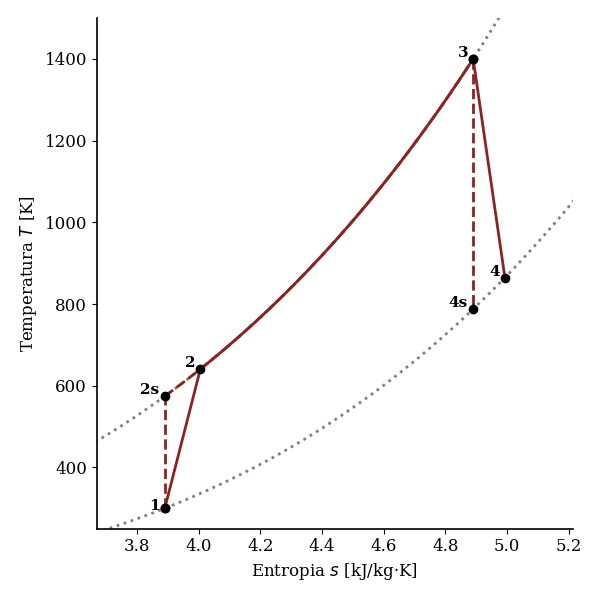
\includegraphics[width=0.45\linewidth]{graphs/brayton-Ts-real.png}
    \caption{Ciclo de Brayton Real}
    \label{fig:brayton-Ts-real}
\end{figure}

No caso real, temos de considerar as irreversibilidades no compressor e na turbina, que terão eficiências isentrópicas, respetivamente, $\eta_c$ e $\eta_t$.

Pode-se pensar que, no compressor, o ideal é fornecer o menor trabalho possível que atinja o objetivo, desta forma o trabalho isentrópico (sem irreversibilidades) será menor que o trabalho real, onde se gera entropia.

Por isso, a eficiência isentrópica do compressor é dado por:

\begin{equation}
    \eta_c = \frac{(\dot{W}_c/\dot{m})_s}{(\dot{W}_c/\dot{m})} = \frac{h_{2s} - h_1}{h_{2} - h_1}
\end{equation}

Por outro lado, na turbina o caso ideal é onde recebemos o maior trabalho possível e, portanto, o trabalho isentrópico será maior que o trabalho real:

\begin{equation}
    \eta_t = \frac{(\dot{W}_t/\dot{m})}{(\dot{W}_t/\dot{m})_s} = \frac{h_3 - h_4}{h_3 - h_{4s}}
\end{equation}

Assim, sabendo as eficiências isentrópicas pode-se calcular os estados reais, normalmente, desconhecidos através de $h_2$ e $h_4$.

Além disso, sendo gás perfeito, temos $h= c_p T$:

\begin{equation}
    \eta_c = \frac{T_{2s} - T_1}{T_{2} - T_1} \qquad \eta_t = \frac{T_3 - T_4}{T_3 - T_{4s}}
\end{equation}

E podemos calcular as incógnitas $T_2$ e $T_4$:

\begin{equation}
    T_2 = T_1 + \frac{T_{2s} - T_1}{\eta_c} \qquad T_4 = T_3 + \eta_t (T_{4s} - T_3) 
\end{equation}

Sendo a eficiência máxima dada por:

\begin{equation}
    \eta_{max} = 1 - \frac{T_1}{T_{2s}} = 1 - \left(\frac{1}{r_p}\right)^{(k-1)/k}
\end{equation}

\subsection{Arrefecimento por andares - Intercooling}

Usando arrefecimento por andares, ou intercooling, consegue-se reduzir o trabalho específico de compressão necessário: $(\dot{W}/\dot{m}) = \int vdp$, pois a menor temperatura, menor o volume específico $v = \frac{RT}{p}$, para a mesma pressão.
Para se atingir esse objetivo, substitui-se o compressor por um dado número de compressores intercalados por radiadores, para arrefecer o ar entre compressões.

No caso de dois compressores dispostos em série — series twin-turbo — o ar é primeiro comprimido até uma pressão intermediária pelo primeiro turbo, depois arrefecido num intercooler, e finalmente comprimido até à pressão final pelo segundo turbo. Idealmente, com múltiplos estágios de compressão e arrefecimento perfeito entre eles, seria possível atingir a pressão final mantendo a temperatura aproximadamente constante, aproximando-se de uma compressão isotérmica (processo $pv=\text{const.}$ para gás ideal), que é mais eficiente do ponto de vista termodinâmico.

\begin{figure}[H]
    \centering
    \begin{subfigure}{0.4\textwidth}
        \centering
        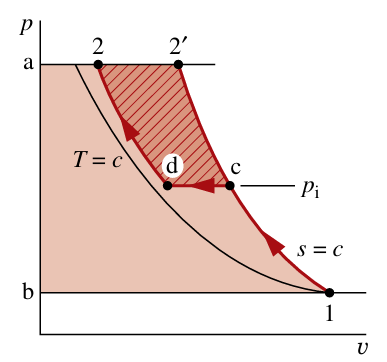
\includegraphics[width=\textwidth]{images/intercooling.png}
        \caption{Compressão em dois estágios com intercooling - Diagrama p-v \cite{shapiro}}
        \label{fig:intercooling}
    \end{subfigure}
    \hfill
    \begin{subfigure}{0.4\textwidth}
        \centering
        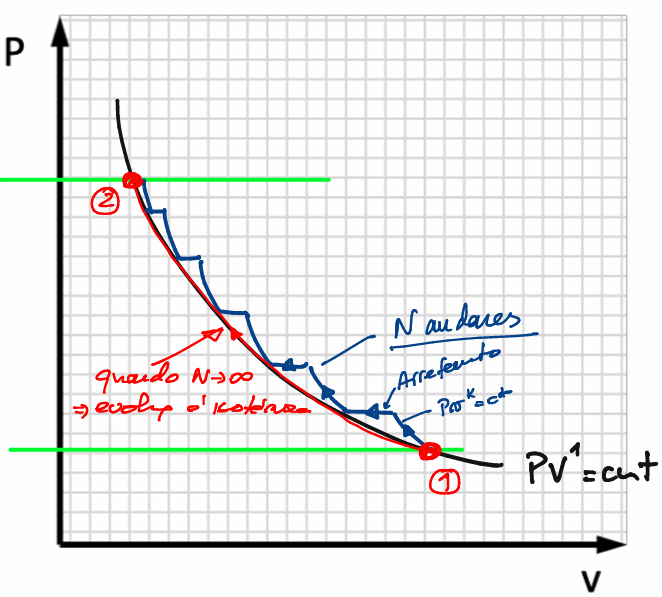
\includegraphics[width=\textwidth]{images/intercooling-isotermico.png}
        \caption{Intercooling ideal - processo isotérmico}
        \label{fig:intercooling-isotermico}
    \end{subfigure}
    \caption{Intercooling - Diagramas p-v}
\end{figure}

Como $\frac{\dot{W}}{\dot{m}} = \int v dp$, o trabalho é a área entre as linhas dos processos $pv^n = \text{const.}$ e o eixo $p$ (pressão) limitado pelas duas linhas horizontais referentes à pressão inicial e final ($p_1$ e $p_2$).

Assim, há uma diminuição do trabalho necessário de compressão necessário entre $p_1$ e $p_2$ ao se arrefecer em estágios intermédios. Além disso, pode-se ver que a área é mínima para o processo isotérmico.


\begin{figure}[H]
    \centering
    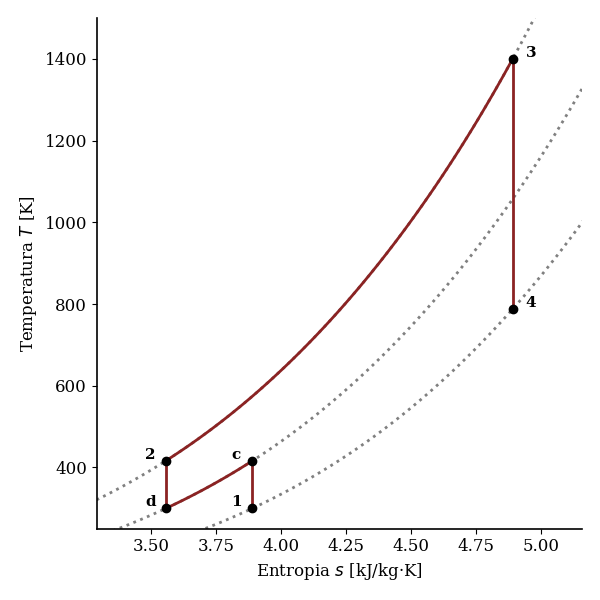
\includegraphics[width=0.45\linewidth]{graphs/brayton-Ts-ideal-intercooling.png}
    \caption{Compressão em dois estágios com intercooling - Diagrama T-s}
    \label{fig:brayton-Ts-ideal-intercooling}
\end{figure}

A pressão intermédia ótima, onde o trabalho de compressão é mínimo, para esta configuração pode ser calculada:

\begin{equation*}
    \frac{\dot{W}}{\dot{m}} = (h_c - h_1) + (h_2 - h_d)
\end{equation*}

onde há uma primeira compressão de 1 para c, arrefecimento de c para d e compressão final de d para 2.

\begin{equation*}
    \frac{\dot{W}}{\dot{m}} = c_p(T_c - T_1) + c_p(T_2 - T_d) = c_p T_1\left(\frac{T_c}{T_1} - 1\right) + c_p T_d \left(\frac{T_2}{T_d} - 1 \right)
\end{equation*}

Considerando compressão isentrópica: $\frac{T_c}{T_1} = \left( \frac{p_i}{p_1} \right)^{(k-1)/k}$ e $\frac{T_2}{T_d} = \left( \frac{p_2}{p_i} \right)^{(k-1)/k}$

\begin{equation*}
    \frac{\dot{W}}{\dot{m}} = c_p T_1\left(\left( \frac{p_i}{p_1} \right)^{(k-1)/k} - 1\right) + c_p T_d \left(\left( \frac{p_2}{p_i} \right)^{(k-1)/k} - 1 \right)
\end{equation*}

\begin{equation*}
    \begin{split}
        \frac{\partial (\dot{W}/ \dot{m})}{\partial p_i} & = c_p T_1 \left( \frac{k-1}{k} \right) \left[ \left( \frac{p_i}{p_1} \right)^{-1/k}  \left( \frac{1}{p_1} \right) - \frac{T_d}{T_1} \left( \frac{p_2}{p_i} \right)^{-1/k} \left( \frac{p_2}{p_i^2} \right) \right] \\
        & = c_p T_1 \left( \frac{k-1}{k} \right) \frac{1}{p_i} \left[ \left( \frac{p_i}{p_1} \right)^{(k-1)/k} - \frac{T_d}{T_1} \left( \frac{p_2}{p_i} \right)^{(k-1)/k} \right]
    \end{split}
\end{equation*}

\begin{eqnarray}
    \frac{\partial (\dot{W}/ \dot{m})}{\partial p_i} = 0 \Longleftrightarrow \left( \frac{p_i}{p_1} \right)^{(k-1)/k} = \frac{T_d}{T_1} \left( \frac{p_2}{p_i} \right)^{(k-1)/k} \nonumber \\ 
    \implies \frac{p_i}{p_1} = \left( \frac{T_d}{T_1}\right)^{k/(k-1)} \frac{p_2}{p_i} \Longleftrightarrow p_i = \sqrt{p_1 p_2 \left( \frac{T_d}{T_1}\right)^{k/(k-1)}}
\end{eqnarray}

Considerando que o arrefecimento permite que $T_d = T_1$, i.e. voltar a comprimir à mesma temperatura, obtemos o valor ótimo de $p_i = \sqrt{p_1 p_2}$.

No caso real, haverá um aumento de entropia na compressão, sendo necessário maior arrefecimento para atingir a pressão desejada a uma temperatura não muito superior à do caso ideal.

\begin{figure}[H]
    \centering
    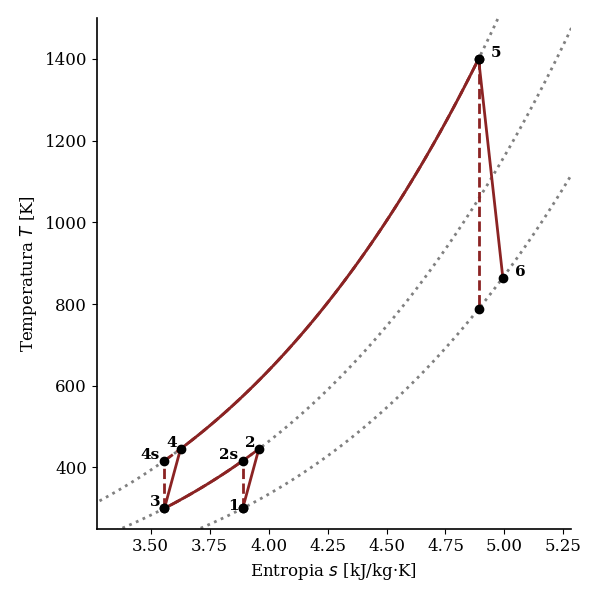
\includegraphics[width=0.45\linewidth]{graphs/brayton-Ts-real-intercooling.png}
    \caption{Ciclo de Brayton Real com Intercooling}
    \label{fig:brayton-Ts-real-intercooling}
\end{figure}


\newgeometry{left=0.5cm, right=1cm, top=0.5cm, bottom=1cm}
\appendix
% \let\cleardoublepage\clearpage
\clearpage
\chapter*{}
\vspace*{-5em} % ajusta conforme o quanto de espaço quer remover
\thispagestyle{empty}
\addcontentsline{toc}{chapter}{Formulário}


\setlength{\columnseprule}{0.5pt}
\def\columnseprulecolor{\color{black}}
\setlength{\columnsep}{1cm}

\setlength{\parindent}{0pt}

\centerline{\Large\textbf{Formulário de Termodinâmica I}}
\footnotesize

\begin{multicols}{2}

\eqn{Constantes}{
&\mathcal{R} = 8.314~\text{kJ/kmol·K} \qquad
N_A = 6.022 \times 10^{23} \qquad R_0 = \frac{\mathcal{R}}{M}\\
&R_{ar} = \frac{\mathcal{R}}{28.97} = 0.287~\text{kJ/kg} \qquad
c_{agua} = 4.186 \ \text{kJ/kg·K} \\
&n = \frac{m}{M} \qquad F = pA \qquad p = p_{atm} + \rho g L \qquad F = \rho g V \\
&\Dot{Q}=kA \nabla T \qquad \Dot{Q}=hA \Delta T \qquad \Dot{Q}=\epsilon \sigma A T^4\\
& h=u+pv \qquad W = - \int p dV \qquad \Dot{W}=Fv \qquad \Dot{m} = pAv
}

\eqn{Conversões}{
&1 \text{ atm} = 101325 \ \text{Pa} = 760 \text{ mmHg}
\qquad 1 \text{ cal} = 4.186 \ \text{J} \\
&1 \text{ Pa} = 1 \text{ N/}\text{m}^2 \qquad
1 \text{ bar} = 10^5 \text{ Pa} \qquad 1 \text{ MPa} = 10 \text{ bar}\\
& T(\text{\textdegree C}) = T(\text{K}) - 273.15 \qquad
T(\text{\textdegree R}) = 1.8 \, T(\text{K}) \\
& T(\text{\textdegree F}) = T(\text{\textdegree R}) - 459.67 \qquad
T(\text{\textdegree F}) = 1.8 \, T(\text{\textdegree C}) + 32
}

\eqn{Balanço de Energia}{
&\Delta E = \Delta E_c + \Delta E_p + \Delta U = Q+W \qquad \frac{dE}{dt} = \Dot{Q} + \Dot{W}\\
&\text{Sistema aberto}:\\
&\frac{dE}{dt} = \Dot{Q} + \Dot{W} + \sum_i \Dot{m_i} \left(\frac{1}{2}v_i^2+gz_i+h_i\right)
}

\eqn{Processo Politrópico}{
&pV^n = pv^n = \text{const} \qquad n = \frac{\ln (p_2 / p_1)}{\ln (V_1 / V_2)} \\
& W= \frac{p_2V_2 - p_1 V_1}{n-1},\ n\neq 1 \qquad W = - p_1 V_1 \ln \frac{V_2}{V_1},\ n=1\\
& n=0 \implies p = \text{const.} \qquad n=\infty \implies v=\text{const.}
}


\eqn{Modelo Gás Ideal}{
&u= u(T) \quad h(T)=u(T)+ RT \quad du = c_p(T) dT \quad dh = c_p(T) dT \\
&c_p =c_v +R \qquad k = \frac{c_p}{c_v} \qquad c_p = \frac{kR}{k-1} \qquad c_v=\frac{R}{k-1}\\
& pv=RT \qquad pV = mRT \qquad pV = n \mathcal{R}T \\
&W = \frac{mR(T_2-T_1)}{n-1},\ n\neq 1 \qquad W = -mRT \ln \frac{V_2}{V_1},\ n=1 \\
&n=1 \Longleftrightarrow \text{isotérmico} \qquad n = k = \frac{c_p}{c_v} \Longleftrightarrow \text{isentrópico} \\
&\frac{T_2}{T_1} = \left( \frac{p_2}{p_1} \right)^{(n-1)/n} = \left( \frac{v_1}{v_2} \right)^{n-1}
}

\eqn{Líquidos}{
&v \approx \text{cte.} \quad \Delta U=mc\Delta T \quad du=dh=c dT \qquad v(T,p) \approx v_f(T) \\
&h(T, P) \approx h_f(T) + v_f(T) (p - p_{sat}(T)) \\
& v = (1-x) v_f + x v_g = v_f + x(v_g - v_f) \qquad \text{Título:} \ x = \frac{m_{vap}}{m} \\
&x = \frac{v-v_f}{v_g-v_f} \qquad y = y_0 + (y_1-y_0) \frac{x-x_0}{x_1-x_0}
}

\eqn{Balanço de Entropia}{
&\Delta S = \int \frac{\delta Q}{T} + \sigma \qquad \frac{dS}{dt} = \int \frac{\Dot{q}}{T} + \sum_i \Dot{m}_i s_i + \Dot{\sigma}\\
&du =Tds -pdv \qquad dh = Tds + vdp \qquad \Delta s = \Delta s^0 - R\ln \frac{p_2}{p_1}
}

\eqn{Trabalho Internalmente Reversível - Sistema Aberto}{
&\left( \frac{\dot{W}}{\dot{m}} \right)_{\substack{\text{int} \\ \text{rev}}} = \int_1^2 v dp \qquad \left( \frac{\dot{W}}{\dot{m}} \right)_{\substack{\text{int} \\ \text{rev}}} = \frac{n}{n-1} \left(p_2 v_2 - p_1 v_1\right), \ n \neq 1\\
&\left( \frac{\dot{W}}{\dot{m}} \right)_{\substack{\text{int} \\ \text{rev}}} = p_1 v_1 \ln \frac{p_2}{p_1} = p_2 v_2 \ln \frac{p_2}{p_1}, \ n = 1\\
&\text{Gás Ideal:}\\
&\left( \frac{\dot{W}}{\dot{m}} \right)_{\substack{\text{int} \\ \text{rev}}} = \frac{n R}{n-1} \left(T_2 - T_1\right), \ n \neq 1 \; \left( \frac{\dot{W}}{\dot{m}} \right)_{\substack{\text{int} \\ \text{rev}}} = RT \ln \frac{p_2}{p_1}, \ n = 1 \\
&\left( \frac{\dot{W}}{\dot{m}} \right)_{\substack{\text{int} \\ \text{rev}}} = \frac{n R}{n-1} T_1 \left[  \left( \frac{p_2}{p_1} \right)^{(n-1)/n} - 1 \right], \ n \neq 1 
}

\eqn{Variação de Entropia}{
&\Delta s = c_v \ln \frac{T_2}{T_1} + R \ln \frac{v_2}{v_1} \qquad \Delta s = c_p \ln \frac{T_2}{T_1} - R \ln \frac{p_2}{p_1} \\
&\Delta s = c_v \ln \frac{p_2}{p_1} + c_p \ln \frac{v_2}{v_1} \qquad \text{Líquido incompressível:}\ \Delta s=c \ln \frac{T_2}{T_1}
}

\eqn{Processos Isentrópicos}{
&s^0(T_2) = s^0(T_1) + R \ln \frac{p_2}{p_1} \\
&\text{Ar:} \ \frac{p_2}{p_1} = \frac{p_{r2}}{p_{r1}} \qquad \frac{v_2}{v_1} = \frac{v_{r2}}{v_{r1}} 
}

\eqn{Ciclos}{
&\text{Condensador e Caldeira - isotérmicos}\\
&\text{Turbina e compressor - abiabáticos}\\
&\eta =\frac{W_u}{Q_H} =  \frac{Q_H- Q_C}{Q_H} = 1 - \frac{Q_C}{Q_H} = 1 - \frac{T_C}{T_H}\\
&\text{COP}_{\text{frig.}} = \beta = \frac{Q_C}{W_{ciclo}} = \frac{Q_C}{Q_H - Q_C} \qquad \beta = \frac{1}{\eta} - 1 \\
&\text{COP}_{\text{bomba}} = \gamma = \frac{Q_H}{W_{ciclo}} = \frac{Q_H}{Q_H - Q_C} \qquad \gamma = \frac{1}{\eta}\\
&\text{bwr} = \frac{\Dot{W}_c / \Dot{m}}{\Dot{W}_t / \Dot{m}} \qquad \text{Válvulas:} \ \Delta h \approx 0, \; \Delta p \propto L
}

\eqn{Ciclo de Brayton}{
&\eta=1 - \frac{h_4 - h_1}{h_3 - h_2} \qquad \eta_{max} = 1 - \frac{T_1}{T_{2s}} = 1 - \left(\frac{1}{r_p}\right)^{(k-1)/k}\\
&T_{2s} = T_1 \left( \frac{p_2}{p_1} \right)^{(k-1)/k} = T_1 \left( r_p \right)^{(k-1)/k} \\
&T_{4s} = T_3 \left( \frac{p_4}{p_3} \right)^{(k-1)/k} = T_3 \left( \frac{1}{r_p} \right)^{(k-1)/k}\\
&\eta_t = \frac{h_4-h_3}{h_{4s}-h_3} = \frac{(\dot{W}_t/\dot{m})}{(\dot{W}_t/\dot{m})_s} \qquad \eta_c = \frac{(\dot{W}_c/\dot{m})_s}{(\dot{W}_c/\dot{m})} = \frac{h_{2s}-h_1}{h_2-h_1}\\
&T_4 = T_3 + \eta_t (T_{4s}-T_3) \qquad T_2 = T_1 + \frac{T_{2s}-T_1}{\eta_c}\\
&\Dot{W}_u \ \text{máximo}: \ r_p = \sqrt{r_{p_{max}}} \\
&\text{Intercooling:} \ p_{int}=\sqrt{p_1 p_2}
}

\end{multicols}

\normalsize
\restoregeometry

\backmatter
\phantomsection
\addcontentsline{toc}{chapter}{Bibliografia}
\begin{thebibliography}{9}
\bibitem{shapiro}
Michael J. Moran and Howard N. Shapiro and Daisie D. Boettner and Margaret B. Bailey (2022), \emph{Fundamentals of Enginnering Thermodynamics - 9th Edition}, Wiley

\end{thebibliography}

\end{document}